\documentclass[9pt]{beamer}

\usetheme{metropolis}

\usepackage{adjustbox}
\usepackage{amssymb}
\usepackage{float}
\usepackage{hyperref}
\usepackage{pgfplots}
\usepackage{pgfplotstable}
%\usepackage{showframe}
\usepackage{subcaption}
\usepackage{tikz}
\usepackage{transparent}
\usepackage{xcolor}

\usepgfplotslibrary{fillbetween}
\usepgfplotslibrary{groupplots}

\usetikzlibrary{arrows.meta}
\usetikzlibrary{calc}
\usetikzlibrary{decorations}
\usetikzlibrary{matrix}

\hypersetup{
    colorlinks=true,
    linkcolor=blue,
	urlcolor=blue
}

\pgfplotsset{compat=1.18}

\def\logoheight{1.2cm}
\def\logosep{0.5cm}

\date{03.07.23}
\title{Midway assessment}
\subtitle{Characterizing the brain using deep neural networks}
\author{Esten H. Leonardsen}

\titlegraphic{
	\centering
	\vspace{7.5cm}
	\includegraphics[height=\logoheight]{data/norment.png}
	\hspace{\logosep}
	\includegraphics[height=\logoheight]{data/lifescience.png}
	\hspace{\logosep}
	\includegraphics[height=\logoheight]{data/lcbc.png}
	\hspace{\logosep}
}
\definecolor{hbn-clr}{RGB}{255, 0, 40}
\definecolor{adhd200-clr}{RGB}{255, 27, 0}
\definecolor{ping-clr}{RGB}{255, 96, 0}
\definecolor{ds000119-clr}{RGB}{255, 165, 0}
\definecolor{abide-clr}{RGB}{255, 234, 0}
\definecolor{slim-clr}{RGB}{206, 255, 0}
\definecolor{abide2-clr}{RGB}{137, 255, 0}
\definecolor{beijing-clr}{RGB}{68, 255, 0}
\definecolor{aomic-clr}{RGB}{0, 255, 0}
\definecolor{corr-clr}{RGB}{0, 255, 68}
\definecolor{mpi-clr}{RGB}{0, 255, 137}
\definecolor{hcp-clr}{RGB}{0, 255, 205}
\definecolor{fcon-clr}{RGB}{0, 235, 255}
\definecolor{nki-clr}{RGB}{0, 166, 255}
\definecolor{sald-clr}{RGB}{0, 97, 255}
\definecolor{ds000222-clr}{RGB}{0, 27, 255}
\definecolor{dlbs-clr}{RGB}{41, 0, 255}
\definecolor{camcan-clr}{RGB}{110, 0, 255}
\definecolor{ukb-clr}{RGB}{180, 0, 255}
\definecolor{oasis-clr}{RGB}{249, 0, 255}
\definecolor{ds000202-clr}{RGB}{255, 0, 191}

\definecolor{conv-clr}{HTML}{FCFF99}
\definecolor{bn-clr}{HTML}{AAFF99}
\definecolor{relu-clr}{HTML}{70F3FF}
\definecolor{pool-clr}{HTML}{A899FF}
\definecolor{conv1x1-clr}{HTML}{FFCC99}
\definecolor{avgpool-clr}{HTML}{FFADFF}
\definecolor{dropout-clr}{HTML}{FF8585}

\definecolor{dataset}{HTML}{AAFF99}
\definecolor{process}{HTML}{70F3FF}
\definecolor{application}{HTML}{A899FF}

\definecolor{delta}{HTML}{FF8585}
\definecolor{model}{rgb}{0.77, 0.84, 0.84}
\definecolor{nodes}{HTML}{AAFF99}
\definecolor{prediction}{HTML}{85B4FF}

\definecolor{base}{HTML}{AAFF99}
\definecolor{lasso}{HTML}{A899FF}
\definecolor{features}{HTML}{FF8585}

\definecolor{cases-default}{HTML}{EB5353}
\definecolor{controls-default}{HTML}{0079FF}
\definecolor{healthy-default}{HTML}{36AE7C}

\definecolor{baseline}{HTML}{FAEAB1}
\definecolor{preds}{HTML}{E5BA73}
\definecolor{maps}{HTML}{C58940}

\definecolor{color0}{rgb}{0.62, 0.004, 0.259}
\definecolor{color1}{rgb}{0.755, 0.154, 0.291}
\definecolor{color2}{rgb}{0.866, 0.29, 0.298}
\definecolor{color3}{rgb}{0.943, 0.406, 0.268}
\definecolor{color4}{rgb}{0.975, 0.557, 0.323}
\definecolor{color5}{rgb}{0.993, 0.709, 0.403}
\definecolor{color6}{rgb}{0.995, 0.832, 0.506}
\definecolor{color7}{rgb}{0.998, 0.926, 0.625}
\definecolor{color8}{rgb}{0.998, 0.999, 0.746}
\definecolor{color9}{rgb}{0.937, 0.975, 0.65}
\definecolor{color10}{rgb}{0.838, 0.935, 0.609}
\definecolor{color11}{rgb}{0.693, 0.876, 0.639}
\definecolor{color12}{rgb}{0.527, 0.811, 0.645}
\definecolor{color13}{rgb}{0.368, 0.725, 0.662}
\definecolor{color14}{rgb}{0.24, 0.582, 0.721}
\definecolor{color15}{rgb}{0.267, 0.441, 0.698}
\definecolor{color16}{rgb}{0.369, 0.31, 0.635}

\definecolor{input}{HTML}{22577A}
\definecolor{first}{HTML}{38A3A5}
\definecolor{second}{HTML}{57CC99}
\definecolor{third}{HTML}{80ED99}
\definecolor{output}{HTML}{C7F9CC}

\pgfplotstableread[col sep=comma]{data/paper1/disorders/MS/baseline_roc.csv}\MSbaselineroc
\pgfplotstableread[col sep=comma]{data/paper1/disorders/MS/delta_roc.csv}\MSdeltaroc
\pgfplotstableread[col sep=comma]{data/paper1/disorders/MS/features_roc.csv}\MSfeaturesroc
\pgfplotstableread[col sep=comma]{data/paper1/disorders/MS/nn_roc.csv}\MSnnroc

\pgfplotstableread[col sep=comma]{data/paper1/disorders/AD/baseline_roc.csv}\ADbaselineroc
\pgfplotstableread[col sep=comma]{data/paper1/disorders/AD/delta_roc.csv}\ADdeltaroc
\pgfplotstableread[col sep=comma]{data/paper1/disorders/AD/features_roc.csv}\ADfeaturesroc
\pgfplotstableread[col sep=comma]{data/paper1/disorders/AD/nn_roc.csv}\ADnnroc

\pgfplotstableread[col sep=comma]{data/paper1/disorders/MCI/baseline_roc.csv}\MCIbaselineroc
\pgfplotstableread[col sep=comma]{data/paper1/disorders/MCI/delta_roc.csv}\MCIdeltaroc
\pgfplotstableread[col sep=comma]{data/paper1/disorders/MCI/features_roc.csv}\MCIfeaturesroc
\pgfplotstableread[col sep=comma]{data/paper1/disorders/MCI/nn_roc.csv}\MCInnroc

\pgfplotstableread[col sep=comma]{data/paper1/disorders/SCZ/baseline_roc.csv}\SCZbaselineroc
\pgfplotstableread[col sep=comma]{data/paper1/disorders/SCZ/delta_roc.csv}\SCZdeltaroc
\pgfplotstableread[col sep=comma]{data/paper1/disorders/SCZ/features_roc.csv}\SCZfeaturesroc
\pgfplotstableread[col sep=comma]{data/paper1/disorders/SCZ/nn_roc.csv}\SCZnnroc

\pgfplotstableread[col sep=comma]{data/paper1/disorders/BD/baseline_roc.csv}\BDbaselineroc
\pgfplotstableread[col sep=comma]{data/paper1/disorders/BD/delta_roc.csv}\BDdeltaroc
\pgfplotstableread[col sep=comma]{data/paper1/disorders/BD/features_roc.csv}\BDfeaturesroc
\pgfplotstableread[col sep=comma]{data/paper1/disorders/BD/nn_roc.csv}\BDnnroc


\pgfplotstableread[col sep=comma]{data/paper1/disorders/PSY/baseline_roc.csv}\PSYbaselineroc
\pgfplotstableread[col sep=comma]{data/paper1/disorders/PSY/delta_roc.csv}\PSYdeltaroc
\pgfplotstableread[col sep=comma]{data/paper1/disorders/PSY/features_roc.csv}\PSYfeaturesroc
\pgfplotstableread[col sep=comma]{data/paper1/disorders/PSY/nn_roc.csv}\PSYnnroc


\pgfplotstableread[col sep=comma]{data/paper1/disorders/DEP/baseline_roc.csv}\DEPbaselineroc
\pgfplotstableread[col sep=comma]{data/paper1/disorders/DEP/delta_roc.csv}\DEPdeltaroc
\pgfplotstableread[col sep=comma]{data/paper1/disorders/DEP/features_roc.csv}\DEPfeaturesroc
\pgfplotstableread[col sep=comma]{data/paper1/disorders/DEP/nn_roc.csv}\DEPnnroc

\pgfplotstableread[col sep=comma]{data/paper1/disorders/MOOD/baseline_roc.csv}\MOODbaselineroc
\pgfplotstableread[col sep=comma]{data/paper1/disorders/MOOD/delta_roc.csv}\MOODdeltaroc
\pgfplotstableread[col sep=comma]{data/paper1/disorders/MOOD/features_roc.csv}\MOODfeaturesroc
\pgfplotstableread[col sep=comma]{data/paper1/disorders/MOOD/nn_roc.csv}\MOODnnroc

\begin{document}
	\begin{frame}
	 	\maketitle
	\end{frame}

	\begin{frame}{Overview of progress}
		\centering
		\begin{itemize}
			\item Paper 1: Published Neuroimage 01.08.22
			\item Paper 2: Published Molecular Psyhiatry 10.05.23
			\item Paper 3: Preprint medRxiv 27.06.23
			\item Paper 4 (pls don't tell Lars): Finishing modelling
		\end{itemize}
	\end{frame}


	\begin{frame}{Introduction} % Group differences
		\centering
		\vfill
		\begin{tikzpicture}
			\node[inner sep=4pt, draw=black, fill=white] (image) {
				\includegraphics[width=10cm]{data/pipeline.jpeg}
			};
			\node[align=center, font=\scriptsize\linespread{1.1}\selectfont] at ($ (image.south) - (0, 0.7) $) {
				"Understanding the impact of preprocessing pipelines on neuroimaging cortical surface analyses.", \\
				Bhagwat et al. 2021, \textit{GigaScience}, \href{https://doi.org/10.1093/gigascience/giaa155}{https://doi.org/10.1093/gigascience/giaa155}
			};
		\end{tikzpicture}
		\vfill
	\end{frame}

	\begin{frame}{Introduction} % Group differences
		\centering
		\vfill
		\begin{tikzpicture}
			\node[inner sep=4pt, draw=black, fill=white] (image) {
				\includegraphics[width=10cm]{data/traditional.jpg}
			};
			\node[align=center, font=\scriptsize\linespread{1.1}\selectfont] at ($ (image.south) - (0, 0.7) $) {
				"Cortical surface abnormalities are different depending on the stage of schizophrenia: A cross-sectional \\
				vertexwise mega-analysis of thickness, area and gyrification.",\\ Rosa et al. 2021, \textit{Schizophrenia Research}, \href{https://doi.org/10.1016/j.schres.2021.08.011}{https://doi.org/10.1016/j.schres.2021.08.011}
			};
		\end{tikzpicture}
		\vfill
	\end{frame}

	\begin{frame}{Introduction} % Little predictive value
		\centering
		\vfill
		\begin{tikzpicture}
			\node[inner sep=4pt, draw=black, fill=white] (image) {
				\includegraphics[width=5cm]{data/wolfers.jpg}
			};
			\node[align=center, font=\scriptsize\linespread{1.1}\selectfont] at ($ (image.south) - (0, 0.7) $) {
				"From estimating activation locality to predicting\\
				disorder: A review of pattern recognition for\\
				neuroimaging-based psychiatric diagnostics.",\\
				Wolfers et al. 2015, \textit{Neuroscience \& Biobehavioral Reviews},\\
				\href{https://doi.org/10.1016/j.neubiorev.2015.08.001}{https://doi.org/10.1016/j.neubiorev.2015.08.001}
			};
		\end{tikzpicture}
		\vfill
	\end{frame}

	\begin{frame}{Introduction} % Assumptions
		\centering
		\vfill
		\begin{tikzpicture}
			\node[inner sep=4pt, draw=black, fill=white] (image) {
				\includegraphics[width=6cm]{data/westlin.jpeg}
			};
			\node[align=center, font=\scriptsize\linespread{1.1}\selectfont] at ($ (image.south) - (0, 0.7) $) {
				"Improving the study of brain-behavior relationships by revisiting\\
				basic assumptions.",\\
				Westlin et al. 2023, \textit{Trends in Cognitive Sciences},\\
				\href{https://doi.org/10.1016/j.tics.2022.12.015}{https://doi.org/10.1016/j.tics.2022.12.015}
			};
		\end{tikzpicture}
		\vfill
	\end{frame}

	\begin{frame}{Introduction} % Simulated data
		\centering
		\vfill

		\begin{tikzpicture}
			\begin{axis}[
				xlabel=\small{Left hippocampus volume},
				ylabel=\small{Right hippocampus volume},
				xtick=\empty,
				ytick=\empty,
				height=7cm,
				width=7cm,
				xmin=-3,
				xmax=15,
				ymin=-4,
				ymax=13,
				clip=false
			]
				\addplot[
					only marks,
					mark=*,
					draw=blue,
					opacity=0.5,
					fill=blue!50
				] table [
					col sep=comma,
					x=control_x,
					y=control_y
				] {data/case_control_points.csv};
				\addplot[
					only marks,
					mark=*,
					draw=red,
					opacity=0.5,
					fill=red!50
				] table [
					col sep=comma,
					x=case_x,
					y=case_y
				] {data/case_control_points.csv};

				\node[
					draw=red,
					fill=red!50,
					circle,
					opacity=0.5,
					inner sep=1.4pt
				] (cases-legend) at (axis cs: 10.3, -3) {};
				\node[anchor=west, text depth=0] at ($ (cases-legend.east) + (-1, 0) $) {\small{Patients}};
				\node[
					draw=blue,
					fill=blue!50,
					circle,
					opacity=0.5,
					inner sep=1.4pt
				] (control-legend) at ($ (cases-legend.north) + (0, 6) $) {};
				\node[anchor=west, text depth=0] at ($ (control-legend.east) + (-1, 0) $) {\small{Controls}};
				\node[] at (axis cs: -5, -5) {};
				\node[] at (axis cs: 19.6, 17.3) {};
			\end{axis}
		\end{tikzpicture}
		\vfill
	\end{frame}

	\begin{frame}{Introduction} % Decision line
		\centering
		\vfill

		\begin{tikzpicture}
			\begin{axis}[
				xlabel=\small{Left hippocampus volume},
				ylabel=\small{Right hippocampus volume},
				xtick=\empty,
				ytick=\empty,
				height=7cm,
				width=7cm,
				xmin=-3,
				xmax=15,
				ymin=-4,
				ymax=13,
				clip=false
			]
				\addplot[
					only marks,
					mark=*,
					draw=blue,
					opacity=0.5,
					fill=blue!50
				] table [
					col sep=comma,
					x=control_x,
					y=control_y
				] {data/case_control_points.csv};
				\addplot[
					only marks,
					mark=*,
					draw=red,
					opacity=0.5,
					fill=red!50
				] table [
					col sep=comma,
					x=case_x,
					y=case_y
				] {data/case_control_points.csv};
				\addplot[dashed] coordinates {
					(-1.7, -3)
					(12.9, 11.6)
				};
				\node[
					draw=red,
					fill=red!50,
					circle,
					opacity=0.5,
					inner sep=1.4pt
				] (cases-legend) at (axis cs: 10.3, -3) {};
				\node[anchor=west, text depth=0] at ($ (cases-legend.east) + (-1, 0) $) {\small{Patients}};
				\node[
					draw=blue,
					fill=blue!50,
					circle,
					opacity=0.5,
					inner sep=1.4pt
				] (control-legend) at ($ (cases-legend.north) + (0, 6) $) {};
				\node[anchor=west, text depth=0] at ($ (control-legend.east) + (-1, 0) $) {\small{Controls}};
				\node[] at (axis cs: -5, -5) {};
				\node[] at (axis cs: 19.6, 17.3) {};
			\end{axis}
		\end{tikzpicture}
		\vfill
	\end{frame}

	\begin{frame}{Introduction} % Group differences
		\newsavebox{\xbox}
		\sbox{\xbox}{%
			\begin{tikzpicture}
				\begin{axis}[
					xmin=-3,
					xmax=16,
					ymin=0,
					ymax=1,
					width=7cm,
					height=3cm,
					axis line style={draw=none},
					tick style={draw=none},
					x dir=reverse,
					xtick=\empty,
					ytick=\empty
				]
					\addplot[draw=none, name path=zero] coordinates {
						(-5.80, 0)
						(17.38, 0)
					};
					\addplot[name path=case,draw=none] table [
						col sep=comma,
						x=x,
						y=case
					] {data/case_control_x_distributions.csv};
					\tikzfillbetween[of=zero and case]{blue, opacity=0.2};
					\addplot[name path=control,draw=none] table [
						col sep=comma,
						x=x,
						y=control
					] {data/case_control_x_distributions.csv};
					\tikzfillbetween[of=zero and control]{red, opacity=0.2};
				\end{axis}
			\end{tikzpicture}
		}


		\newsavebox{\ybox}
		\sbox{\ybox}{%
			\begin{tikzpicture}
				\begin{axis}[
					xmin=-5,
					xmax=15,
					ymin=0,
					ymax=1,
					width=7cm,
					height=3cm,
					axis line style={draw=none},
					tick style={draw=none},
					xtick=\empty,
					ytick=\empty
				]
					\addplot[draw=none, name path=zero] coordinates {
						(-5.80, 0)
						(17.38, 0)
					};
					\addplot[name path=case,draw=none] table [
						col sep=comma,
						x=y,
						y=case
					] {data/case_control_y_distributions.csv};
					\tikzfillbetween[of=zero and case]{blue, opacity=0.2};
					\addplot[name path=control,draw=none] table [
						col sep=comma,
						x=y,
						y=control
					] {data/case_control_y_distributions.csv};
					\tikzfillbetween[of=zero and control]{red, opacity=0.2};
				\end{axis}
			\end{tikzpicture}
		}

		\centering
		\vfill

		\begin{tikzpicture}
			\begin{axis}[
				xlabel=\small{Left hippocampus volume},
				ylabel=\small{Right hippocampus volume},
				xtick=\empty,
				ytick=\empty,
				height=7cm,
				width=7cm,
				xmin=-3,
				xmax=15,
				ymin=-4,
				ymax=13,
				clip=false
			]
				\addplot[
					only marks,
					mark=*,
					draw=blue,
					opacity=0.5,
					fill=blue!50
				] table [
					col sep=comma,
					x=control_x,
					y=control_y
				] {data/case_control_points.csv};
				\addplot[
					only marks,
					mark=*,
					draw=red,
					opacity=0.5,
					fill=red!50
				] table [
					col sep=comma,
					x=case_x,
					y=case_y
				] {data/case_control_points.csv};
				\addplot[dashed] coordinates {
					(-1.7, -3)
					(12.9, 11.6)
				};
				\node[anchor=south,rotate=270, inner sep=0pt, outer sep=0pt] at (axis cs: 15, 4.454) {\usebox{\xbox}};
				\node[anchor=south, inner sep=0pt, outer sep=0pt] at (axis cs: 6.15, 13) {\usebox{\ybox}};
				\node[
					draw=red,
					fill=red!50,
					circle,
					opacity=0.5,
					inner sep=1.4pt
				] (cases-legend) at (axis cs: 10.3, -3) {};
				\node[anchor=west, text depth=0] at ($ (cases-legend.east) + (-1, 0) $) {\small{Patients}};
				\node[
					draw=blue,
					fill=blue!50,
					circle,
					opacity=0.5,
					inner sep=1.4pt
				] (control-legend) at ($ (cases-legend.north) + (0, 6) $) {};
				\node[anchor=west, text depth=0] at ($ (control-legend.east) + (-1, 0) $) {\small{Controls}};
				\node[] at (axis cs: -5, -5) {};
				\node[] at (axis cs: 19.6, 17.3) {};
			\end{axis}
		\end{tikzpicture}
		\vfill
	\end{frame}

	\begin{frame}{Introduction} % GLM
		\centering
		\vfill
		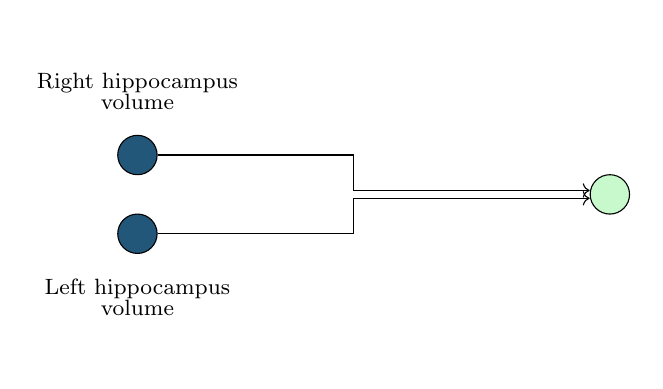
\begin{tikzpicture}
			\node[
				draw=black,
				fill=input,
				circle,
				minimum size=0.5cm,
				label={[align=center, font=\footnotesize\linespread{0.8}\selectfont, label distance=0.2cm]above:{Right hippocampus\\volume}}
			] (in1)at (0, 0) {};
			\node[
				draw=black,
				fill=input,
				circle,
				minimum size=0.5cm,
				label={[align=center, font=\footnotesize\linespread{0.8}\selectfont, label distance=0.2cm]below:{Left hippocampus\\volume}}
			] (in2) at (0, -1) {};

			\node[
				draw=black,
				minimum size=0.5cm,
				circle,
				fill=output
			] (out) at (6, -0.5) {};

			\draw[->] (in1) -| ($ (out.west) - (3, -0.05) $) -- ($ (out.west) + (0, 0.05) $);
			\draw[->] (in2) -| ($ (out.west) - (3, 0.05) $) -- ($ (out.west) + (0, -0.05) $);

			\node[] at (-0.9, -2.5) {};
			\node[] at (6.2, 1.5) {};
		\end{tikzpicture}
		\vfill
	\end{frame}

	\begin{frame}{Introduction} % Interaction
		\centering
		\vfill
		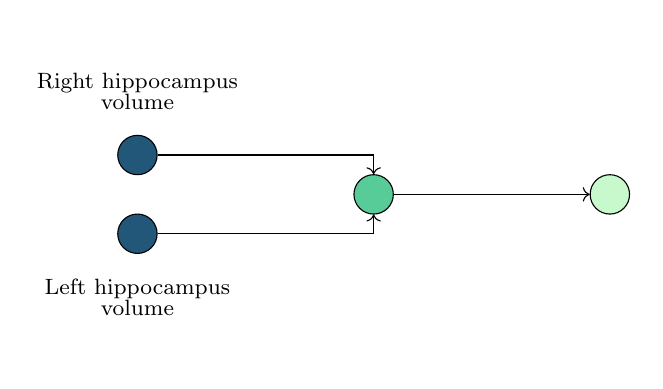
\begin{tikzpicture}
			\node[
				draw=black,
				fill=input,
				circle,
				minimum size=0.5cm,
				label={[align=center, font=\footnotesize\linespread{0.8}\selectfont, label distance=0.2cm]above:{Right hippocampus\\volume}}
			] (in1)at (0, 0) {};
			\node[
				draw=black,
				fill=input,
				circle,
				minimum size=0.5cm,
				label={[align=center, font=\footnotesize\linespread{0.8}\selectfont, label distance=0.2cm]below:{Left hippocampus\\volume}}
			] (in2) at (0, -1) {};


			\node[
				draw=black,
				minimum size=0.5cm,
				circle,
				fill=second
			] (n10) at (3, -0.5) {};

			\node[
				draw=black,
				minimum size=0.5cm,
				circle,
				fill=output
			] (out) at (6, -0.5) {};

			\draw[->] (in1) -| (n10.north);
			\draw[->] (in2) -| (n10.south);
			\draw[->] (n10) -- (out);

			\node[] at (-0.9, -2.5) {};
			\node[] at (6.2, 1.5) {};
		\end{tikzpicture}
		\vfill
	\end{frame}

	\begin{frame}{Introduction} % Neural network
		\centering
		\vfill
		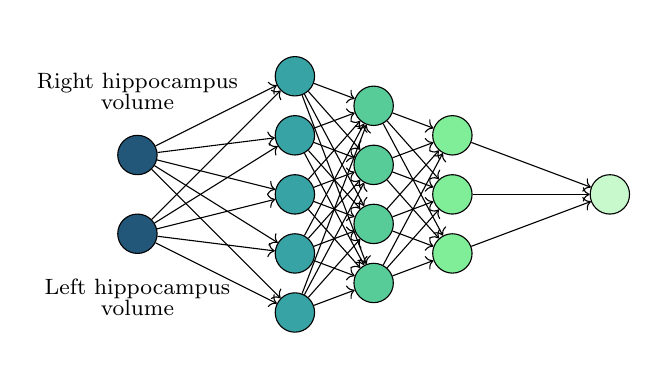
\begin{tikzpicture}
			\node[
				draw=black,
				fill=input,
				circle,
				minimum size=0.5cm,
				label={[align=center, font=\footnotesize\linespread{0.8}\selectfont, label distance=0.2cm]above:{Right hippocampus\\volume}}
			] (in1)at (0, 0) {};
			\node[
				draw=black,
				fill=input,
				circle,
				minimum size=0.5cm,
				label={[align=center, font=\footnotesize\linespread{0.8}\selectfont, label distance=0.2cm]below:{Left hippocampus\\volume}}
			] (in2) at (0, -1) {};

			\node[
				draw=black,
				minimum size=0.5cm,
				circle,
				fill=first
			] (n00) at (2, 1) {};
			\node[
				draw=black,
				minimum size=0.5cm,
				circle,
				fill=first
			] (n01) at (2, 0.25) {};
			\node[
				draw=black,
				minimum size=0.5cm,
				circle,
				fill=first
			] (n02) at (2, -0.5) {};
			\node[
				draw=black,
				minimum size=0.5cm,
				circle,
				fill=first
			] (n03) at (2, -1.25) {};
			\node[
				draw=black,
				minimum size=0.5cm,
				circle,
				fill=first
			] (n04) at (2, -2) {};

			\node[
				draw=black,
				minimum size=0.5cm,
				circle,
				fill=second
			] (n10) at (3, 0.625) {};
			\node[
				draw=black,
				minimum size=0.5cm,
				circle,
				fill=second
			] (n11) at (3, -0.125) {};
			\node[
				draw=black,
				minimum size=0.5cm,
				circle,
				fill=second
			] (n12) at (3, -0.875) {};
			\node[
				draw=black,
				minimum size=0.5cm,
				circle,
				fill=second
			] (n13) at (3, -1.625) {};

			\node[
				draw=black,
				minimum size=0.5cm,
				circle,
				fill=third
			] (n20) at (4, 0.25) {};
			\node[
				draw=black,
				minimum size=0.5cm,
				circle,
				fill=third
			] (n21) at (4, -0.5) {};
			\node[
				draw=black,
				minimum size=0.5cm,
				circle,
				fill=third
			] (n22) at (4, -1.25) {};

			\node[
				draw=black,
				minimum size=0.5cm,
				circle,
				fill=output
			] (out) at (6, -0.5) {};

			\draw[->] (in1) -- (n00);
			\draw[->] (in1) -- (n01);
			\draw[->] (in1) -- (n02);
			\draw[->] (in1) -- (n03);
			\draw[->] (in1) -- (n04);

			\draw[->] (in2) -- (n00);
			\draw[->] (in2) -- (n01);
			\draw[->] (in2) -- (n02);
			\draw[->] (in2) -- (n03);
			\draw[->] (in2) -- (n04);

			\draw[->] (n00) -- (n10);
			\draw[->] (n00) -- (n11);
			\draw[->] (n00) -- (n12);
			\draw[->] (n00) -- (n13);

			\draw[->] (n01) -- (n10);
			\draw[->] (n01) -- (n11);
			\draw[->] (n01) -- (n12);
			\draw[->] (n01) -- (n13);

			\draw[->] (n02) -- (n10);
			\draw[->] (n02) -- (n11);
			\draw[->] (n02) -- (n12);
			\draw[->] (n02) -- (n13);

			\draw[->] (n03) -- (n10);
			\draw[->] (n03) -- (n11);
			\draw[->] (n03) -- (n12);
			\draw[->] (n03) -- (n13);

			\draw[->] (n04) -- (n10);
			\draw[->] (n04) -- (n11);
			\draw[->] (n04) -- (n12);
			\draw[->] (n04) -- (n13);

			\draw[->] (n10) -- (n20);
			\draw[->] (n10) -- (n21);
			\draw[->] (n10) -- (n22);

			\draw[->] (n11) -- (n20);
			\draw[->] (n11) -- (n21);
			\draw[->] (n11) -- (n22);

			\draw[->] (n12) -- (n20);
			\draw[->] (n12) -- (n21);
			\draw[->] (n12) -- (n22);

			\draw[->] (n13) -- (n20);
			\draw[->] (n13) -- (n21);
			\draw[->] (n13) -- (n22);

			\draw[->] (n20) -- (out);
			\draw[->] (n21) -- (out);
			\draw[->] (n22) -- (out);

			\node[] at (-0.9, -2.5) {};
			\node[] at (6.2, 1.5) {};
		\end{tikzpicture}
		\vfill
	\end{frame}

	\begin{frame}{Introduction} % Neural network
		\centering
		\vfill
		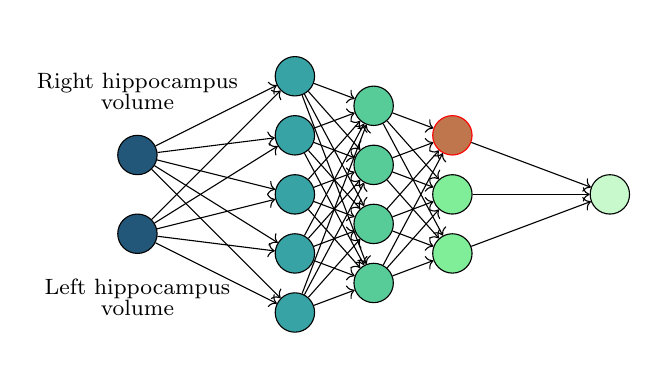
\begin{tikzpicture}
			\node[
				draw=black,
				fill=input,
				circle,
				minimum size=0.5cm,
				label={[align=center, font=\footnotesize\linespread{0.8}\selectfont, label distance=0.2cm]above:{Right hippocampus\\volume}}
			] (in1)at (0, 0) {};
			\node[
				draw=black,
				fill=input,
				circle,
				minimum size=0.5cm,
				label={[align=center, font=\footnotesize\linespread{0.8}\selectfont, label distance=0.2cm]below:{Left hippocampus\\volume}}
			] (in2) at (0, -1) {};

			\node[
				draw=black,
				minimum size=0.5cm,
				circle,
				fill=first
			] (n00) at (2, 1) {};
			\node[
				draw=black,
				minimum size=0.5cm,
				circle,
				fill=first
			] (n01) at (2, 0.25) {};
			\node[
				draw=black,
				minimum size=0.5cm,
				circle,
				fill=first
			] (n02) at (2, -0.5) {};
			\node[
				draw=black,
				minimum size=0.5cm,
				circle,
				fill=first
			] (n03) at (2, -1.25) {};
			\node[
				draw=black,
				minimum size=0.5cm,
				circle,
				fill=first
			] (n04) at (2, -2) {};

			\node[
				draw=black,
				minimum size=0.5cm,
				circle,
				fill=second
			] (n10) at (3, 0.625) {};
			\node[
				draw=black,
				minimum size=0.5cm,
				circle,
				fill=second
			] (n11) at (3, -0.125) {};
			\node[
				draw=black,
				minimum size=0.5cm,
				circle,
				fill=second
			] (n12) at (3, -0.875) {};
			\node[
				draw=black,
				minimum size=0.5cm,
				circle,
				fill=second
			] (n13) at (3, -1.625) {};

			\node[
				draw=red,
				minimum size=0.5cm,
				circle,
				fill=third!50!red
			] (n20) at (4, 0.25) {};
			\node[
				draw=black,
				minimum size=0.5cm,
				circle,
				fill=third
			] (n21) at (4, -0.5) {};
			\node[
				draw=black,
				minimum size=0.5cm,
				circle,
				fill=third
			] (n22) at (4, -1.25) {};

			\node[
				draw=black,
				minimum size=0.5cm,
				circle,
				fill=output
			] (out) at (6, -0.5) {};

			\draw[->] (in1) -- (n00);
			\draw[->] (in1) -- (n01);
			\draw[->] (in1) -- (n02);
			\draw[->] (in1) -- (n03);
			\draw[->] (in1) -- (n04);

			\draw[->] (in2) -- (n00);
			\draw[->] (in2) -- (n01);
			\draw[->] (in2) -- (n02);
			\draw[->] (in2) -- (n03);
			\draw[->] (in2) -- (n04);

			\draw[->] (n00) -- (n10);
			\draw[->] (n00) -- (n11);
			\draw[->] (n00) -- (n12);
			\draw[->] (n00) -- (n13);

			\draw[->] (n01) -- (n10);
			\draw[->] (n01) -- (n11);
			\draw[->] (n01) -- (n12);
			\draw[->] (n01) -- (n13);

			\draw[->] (n02) -- (n10);
			\draw[->] (n02) -- (n11);
			\draw[->] (n02) -- (n12);
			\draw[->] (n02) -- (n13);

			\draw[->] (n03) -- (n10);
			\draw[->] (n03) -- (n11);
			\draw[->] (n03) -- (n12);
			\draw[->] (n03) -- (n13);

			\draw[->] (n04) -- (n10);
			\draw[->] (n04) -- (n11);
			\draw[->] (n04) -- (n12);
			\draw[->] (n04) -- (n13);

			\draw[->] (n10) -- (n20);
			\draw[->] (n10) -- (n21);
			\draw[->] (n10) -- (n22);

			\draw[->] (n11) -- (n20);
			\draw[->] (n11) -- (n21);
			\draw[->] (n11) -- (n22);

			\draw[->] (n12) -- (n20);
			\draw[->] (n12) -- (n21);
			\draw[->] (n12) -- (n22);

			\draw[->] (n13) -- (n20);
			\draw[->] (n13) -- (n21);
			\draw[->] (n13) -- (n22);

			\draw[->] (n20) -- (out);
			\draw[->] (n21) -- (out);
			\draw[->] (n22) -- (out);

			\node[] at (-0.9, -2.5) {};
			\node[] at (6.2, 1.5) {};
		\end{tikzpicture}
		\vfill
	\end{frame}

	\begin{frame}{Introduction} % Neural network
		\centering
		\vfill
		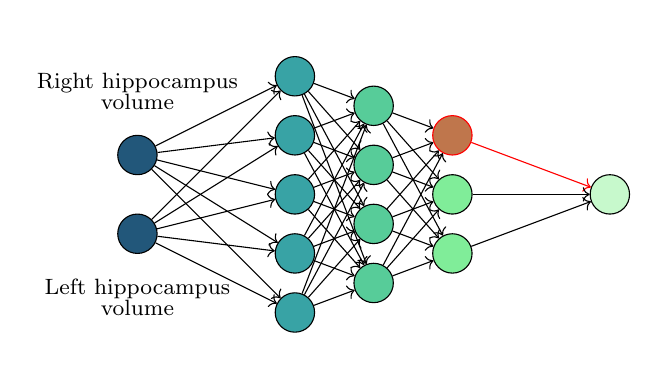
\begin{tikzpicture}
			\node[
				draw=black,
				fill=input,
				circle,
				minimum size=0.5cm,
				label={[align=center, font=\footnotesize\linespread{0.8}\selectfont, label distance=0.2cm]above:{Right hippocampus\\volume}}
			] (in1)at (0, 0) {};
			\node[
				draw=black,
				fill=input,
				circle,
				minimum size=0.5cm,
				label={[align=center, font=\footnotesize\linespread{0.8}\selectfont, label distance=0.2cm]below:{Left hippocampus\\volume}}
			] (in2) at (0, -1) {};

			\node[
				draw=black,
				minimum size=0.5cm,
				circle,
				fill=first
			] (n00) at (2, 1) {};
			\node[
				draw=black,
				minimum size=0.5cm,
				circle,
				fill=first
			] (n01) at (2, 0.25) {};
			\node[
				draw=black,
				minimum size=0.5cm,
				circle,
				fill=first
			] (n02) at (2, -0.5) {};
			\node[
				draw=black,
				minimum size=0.5cm,
				circle,
				fill=first
			] (n03) at (2, -1.25) {};
			\node[
				draw=black,
				minimum size=0.5cm,
				circle,
				fill=first
			] (n04) at (2, -2) {};

			\node[
				draw=black,
				minimum size=0.5cm,
				circle,
				fill=second
			] (n10) at (3, 0.625) {};
			\node[
				draw=black,
				minimum size=0.5cm,
				circle,
				fill=second
			] (n11) at (3, -0.125) {};
			\node[
				draw=black,
				minimum size=0.5cm,
				circle,
				fill=second
			] (n12) at (3, -0.875) {};
			\node[
				draw=black,
				minimum size=0.5cm,
				circle,
				fill=second
			] (n13) at (3, -1.625) {};

			\node[
				draw=red,
				minimum size=0.5cm,
				circle,
				fill=third!50!red
			] (n20) at (4, 0.25) {};
			\node[
				draw=black,
				minimum size=0.5cm,
				circle,
				fill=third
			] (n21) at (4, -0.5) {};
			\node[
				draw=black,
				minimum size=0.5cm,
				circle,
				fill=third
			] (n22) at (4, -1.25) {};

			\node[
				draw=black,
				minimum size=0.5cm,
				circle,
				fill=output
			] (out) at (6, -0.5) {};

			\draw[->] (in1) -- (n00);
			\draw[->] (in1) -- (n01);
			\draw[->] (in1) -- (n02);
			\draw[->] (in1) -- (n03);
			\draw[->] (in1) -- (n04);

			\draw[->] (in2) -- (n00);
			\draw[->] (in2) -- (n01);
			\draw[->] (in2) -- (n02);
			\draw[->] (in2) -- (n03);
			\draw[->] (in2) -- (n04);

			\draw[->] (n00) -- (n10);
			\draw[->] (n00) -- (n11);
			\draw[->] (n00) -- (n12);
			\draw[->] (n00) -- (n13);

			\draw[->] (n01) -- (n10);
			\draw[->] (n01) -- (n11);
			\draw[->] (n01) -- (n12);
			\draw[->] (n01) -- (n13);

			\draw[->] (n02) -- (n10);
			\draw[->] (n02) -- (n11);
			\draw[->] (n02) -- (n12);
			\draw[->] (n02) -- (n13);

			\draw[->] (n03) -- (n10);
			\draw[->] (n03) -- (n11);
			\draw[->] (n03) -- (n12);
			\draw[->] (n03) -- (n13);

			\draw[->] (n04) -- (n10);
			\draw[->] (n04) -- (n11);
			\draw[->] (n04) -- (n12);
			\draw[->] (n04) -- (n13);

			\draw[->] (n10) -- (n20);
			\draw[->] (n10) -- (n21);
			\draw[->] (n10) -- (n22);

			\draw[->] (n11) -- (n20);
			\draw[->] (n11) -- (n21);
			\draw[->] (n11) -- (n22);

			\draw[->] (n12) -- (n20);
			\draw[->] (n12) -- (n21);
			\draw[->] (n12) -- (n22);

			\draw[->] (n13) -- (n20);
			\draw[->] (n13) -- (n21);
			\draw[->] (n13) -- (n22);

			\draw[red,->] (n20) -- (out);
			\draw[->] (n21) -- (out);
			\draw[->] (n22) -- (out);

			\node[] at (-0.9, -2.5) {};
			\node[] at (6.2, 1.5) {};
		\end{tikzpicture}
		\vfill
	\end{frame}

	\begin{frame}{Introduction} % Black box
		\centering
		\vfill
		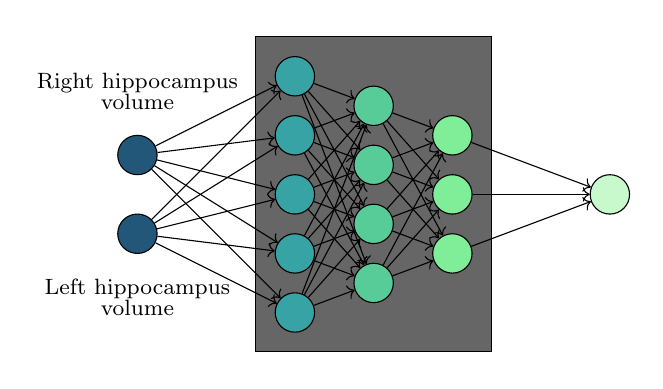
\begin{tikzpicture}
			% Box which emcopasses the nodes in the three middle layers
			\draw[draw=black, fill=black!60] (1.5, -2.5) rectangle (4.5, 1.5);
			\node[
				draw=black,
				fill=input,
				circle,
				minimum size=0.5cm,
				label={[align=center, font=\footnotesize\linespread{0.8}\selectfont, label distance=0.2cm]above:{Right hippocampus\\volume}}
			] (in1)at (0, 0) {};
			\node[
				draw=black,
				fill=input,
				circle,
				minimum size=0.5cm,
				label={[align=center, font=\footnotesize\linespread{0.8}\selectfont, label distance=0.2cm]below:{Left hippocampus\\volume}}
			] (in2) at (0, -1) {};

			\node[
				draw=black,
				minimum size=0.5cm,
				circle,
				fill=first
			] (n00) at (2, 1) {};
			\node[
				draw=black,
				minimum size=0.5cm,
				circle,
				fill=first
			] (n01) at (2, 0.25) {};
			\node[
				draw=black,
				minimum size=0.5cm,
				circle,
				fill=first
			] (n02) at (2, -0.5) {};
			\node[
				draw=black,
				minimum size=0.5cm,
				circle,
				fill=first
			] (n03) at (2, -1.25) {};
			\node[
				draw=black,
				minimum size=0.5cm,
				circle,
				fill=first
			] (n04) at (2, -2) {};

			\node[
				draw=black,
				minimum size=0.5cm,
				circle,
				fill=second
			] (n10) at (3, 0.625) {};
			\node[
				draw=black,
				minimum size=0.5cm,
				circle,
				fill=second
			] (n11) at (3, -0.125) {};
			\node[
				draw=black,
				minimum size=0.5cm,
				circle,
				fill=second
			] (n12) at (3, -0.875) {};
			\node[
				draw=black,
				minimum size=0.5cm,
				circle,
				fill=second
			] (n13) at (3, -1.625) {};

			\node[
				draw=black,
				minimum size=0.5cm,
				circle,
				fill=third
			] (n20) at (4, 0.25) {};
			\node[
				draw=black,
				minimum size=0.5cm,
				circle,
				fill=third
			] (n21) at (4, -0.5) {};
			\node[
				draw=black,
				minimum size=0.5cm,
				circle,
				fill=third
			] (n22) at (4, -1.25) {};

			\node[
				draw=black,
				minimum size=0.5cm,
				circle,
				fill=output
			] (out) at (6, -0.5) {};

			\draw[->] (in1) -- (n00);
			\draw[->] (in1) -- (n01);
			\draw[->] (in1) -- (n02);
			\draw[->] (in1) -- (n03);
			\draw[->] (in1) -- (n04);

			\draw[->] (in2) -- (n00);
			\draw[->] (in2) -- (n01);
			\draw[->] (in2) -- (n02);
			\draw[->] (in2) -- (n03);
			\draw[->] (in2) -- (n04);

			\draw[->] (n00) -- (n10);
			\draw[->] (n00) -- (n11);
			\draw[->] (n00) -- (n12);
			\draw[->] (n00) -- (n13);

			\draw[->] (n01) -- (n10);
			\draw[->] (n01) -- (n11);
			\draw[->] (n01) -- (n12);
			\draw[->] (n01) -- (n13);

			\draw[->] (n02) -- (n10);
			\draw[->] (n02) -- (n11);
			\draw[->] (n02) -- (n12);
			\draw[->] (n02) -- (n13);

			\draw[->] (n03) -- (n10);
			\draw[->] (n03) -- (n11);
			\draw[->] (n03) -- (n12);
			\draw[->] (n03) -- (n13);

			\draw[->] (n04) -- (n10);
			\draw[->] (n04) -- (n11);
			\draw[->] (n04) -- (n12);
			\draw[->] (n04) -- (n13);

			\draw[->] (n10) -- (n20);
			\draw[->] (n10) -- (n21);
			\draw[->] (n10) -- (n22);

			\draw[->] (n11) -- (n20);
			\draw[->] (n11) -- (n21);
			\draw[->] (n11) -- (n22);

			\draw[->] (n12) -- (n20);
			\draw[->] (n12) -- (n21);
			\draw[->] (n12) -- (n22);

			\draw[->] (n13) -- (n20);
			\draw[->] (n13) -- (n21);
			\draw[->] (n13) -- (n22);

			\draw[->] (n20) -- (out);
			\draw[->] (n21) -- (out);
			\draw[->] (n22) -- (out);

			\node[] at (-0.9, -2.5) {};
			\node[] at (6.2, 1.5) {};
		\end{tikzpicture}
		\vfill
	\end{frame}

	\begin{frame}{Introduction}
		\begin{itemize}
			\item There are high level abstractions that could help delineate the relationship between the brain as represented in neuroimaging data and mental and neurological conditions.
			\item Deep neural networks epitomize the expressive capacity to learn and utilize these abstractions.
			\item Approaches need to allow for interpretations of the abstractions themselves.
		\end{itemize}
	\end{frame}

	\begin{frame}{Paper 1: Brain age} % Title
		\centering
		\vfill
		\begin{tikzpicture}
			\node[inner sep=1pt, fill=white, draw=black] {
				\includegraphics[width=8cm]{data/paper1.png}
			};
		\end{tikzpicture}
		\vfill
	\end{frame}

	\begin{frame}{Paper 1: Brain age} % Dataset
		\centering
		\vfill
		\begin{tikzpicture}
			\begin{axis}[
				width=0.9\textwidth,
				height=0.65\textwidth,
				xmin=0,
				xmax=100,
				ymin=-1200,
				ymax=1200,
				yticklabels={,,},
				ytick=\empty,
				xtick pos=bottom,
				y dir=reverse,
				axis x line=middle,
				axis y line=none,
				xtick={0,10,20,30,40,50,60,70,80}
			]
				\addplot [draw=none, name path=zero] coordinates {
					(0, 0)
					(100, 0)
				};

				\addplot [draw=none, name path=hbn] table [col sep=comma, x=age,y=hbn] {data/paper1/dataset/M.csv};
				\addplot [hbn-clr] fill between [of=zero and hbn];
				\addplot [draw=none, name path=adhd200] table [col sep=comma, x=age,y=adhd200-hc] {data/paper1/dataset/M.csv};
				\addplot [adhd200-clr] fill between [of=hbn and adhd200];\label{trace:adhd200}
				\addplot [draw=none, name path=ping] table [col sep=comma, x=age,y=ping] {data/paper1/dataset/M.csv};
				\addplot [ping-clr] fill between [of=adhd200 and ping];\label{trace:ping}

				\addplot [draw=none, name path=ds000119] table [col sep=comma, x=age,y=ds000119] {data/paper1/dataset/M.csv};
				\addplot [ds000119-clr] fill between [of=ping and ds000119];\label{trace:ds000119}
				\addplot [draw=none, name path=abide] table [col sep=comma, x=age,y=abide-hc] {data/paper1/dataset/M.csv};
				\addplot [abide-clr] fill between [of=ds000119 and abide];\label{trace:abide}
				\addplot [draw=none, name path=slim] table [col sep=comma, x=age,y=slim] {data/paper1/dataset/M.csv};
				\addplot [slim-clr] fill between [of=abide and slim];\label{trace:slim}
				\addplot [draw=none, name path=abide2] table [col sep=comma, x=age,y=abide2-hc] {data/paper1/dataset/M.csv};
				\addplot [abide2-clr] fill between [of=slim and abide2];\label{trace:abide2}
				\addplot [draw=none, name path=beijing] table [col sep=comma, x=age,y=beijing-enhanced] {data/paper1/dataset/M.csv};
				\addplot [beijing-clr] fill between [of=slim and beijing];\label{trace:beijing}
				\addplot [draw=none, name path=aomic] table [col sep=comma, x=age,y=aomic-id1000] {data/paper1/dataset/M.csv};
				\addplot [aomic-clr] fill between [of=beijing and aomic];\label{trace:aomic}
				\addplot [draw=none, name path=corr] table [col sep=comma, x=age,y=corr] {data/paper1/dataset/M.csv};
				\addplot [corr-clr] fill between [of=aomic and corr];\label{trace:corr}
				\addplot [draw=none, name path=mpi] table [col sep=comma, x=age,y=mpi-lemon] {data/paper1/dataset/M.csv};
				\addplot [mpi-clr] fill between [of=corr and mpi];\label{trace:mpi}
				\addplot [draw=none, name path=hcp] table [col sep=comma, x=age,y=hcp] {data/paper1/dataset/M.csv};
				\addplot [hcp-clr] fill between [of=mpi and hcp];\label{trace:hcp}
				\addplot [draw=none, name path=fcon] table [col sep=comma, x=age,y=fcon1000] {data/paper1/dataset/M.csv};
				\addplot [fcon-clr] fill between [of=hcp and fcon];\label{trace:fcon}
				\addplot [draw=none, name path=nki] table [col sep=comma, x=age,y=nki-rockland] {data/paper1/dataset/M.csv};
				\addplot [nki-clr] fill between [of=fcon and nki];\label{trace:nki}
				\addplot [draw=none, name path=sald] table [col sep=comma, x=age,y=sald] {data/paper1/dataset/M.csv};
				\addplot [sald-clr] fill between [of=nki and sald];\label{trace:sald}
				\addplot [draw=none, name path=ds000222] table [col sep=comma, x=age,y=ds000222] {data/paper1/dataset/M.csv};
				\addplot [ds000222-clr] fill between [of=sald and ds000222];\label{trace:ds000222}
				\addplot [draw=none, name path=dlbs] table [col sep=comma, x=age,y=dlbs] {data/paper1/dataset/M.csv};
				\addplot [dlbs-clr] fill between [of=ds000222 and dlbs];\label{trace:dlbs}
				\addplot [draw=none, name path=camcan] table [col sep=comma, x=age,y=camcan] {data/paper1/dataset/M.csv};
				\addplot [camcan-clr] fill between [of=dlbs and camcan];\label{trace:camcan}
				\addplot [draw=none, name path=ukb] table [col sep=comma, x=age,y=ukb] {data/paper1/dataset/M.csv};
				\addplot [ukb-clr] fill between [of=camcan and ukb];\label{trace:ukb}
				\addplot [draw=black, name path=oasis] table [col sep=comma, x=age,y=oasis3-hc] {data/paper1/dataset/M.csv};
				\addplot [oasis-clr] fill between [of=ukb and oasis];\label{trace:oasis}

				\addplot [draw=none, name path=hbn] table [col sep=comma, x=age,y expr=\thisrow{hbn}*-1] {data/paper1/dataset/F.csv};
				\addplot [hbn-clr] fill between [of=zero and hbn];\label{trace:hbn}
				\addplot [draw=none, name path=adhd200] table [col sep=comma, x=age,y=,y expr=\thisrow{adhd200-hc}*-1] {data/paper1/dataset/F.csv};
				\addplot [adhd200-clr] fill between [of=hbn and adhd200];
				\addplot [draw=none, name path=ping] table [col sep=comma, x=age,y expr=\thisrow{ping}*-1] {data/paper1/dataset/F.csv};
				\addplot [ping-clr] fill between [of=adhd200 and ping];
				\addplot [draw=none, name path=abide] table [col sep=comma, x=age,y expr=\thisrow{abide-hc}*-1] {data/paper1/dataset/F.csv};
				\addplot [abide-clr] fill between [of=ping and abide];
				\addplot [draw=none, name path=abide2] table [col sep=comma, x=age,y expr=\thisrow{abide2-hc}*-1] {data/paper1/dataset/F.csv};
				\addplot [abide2-clr] fill between [of=abide and abide2];
				\addplot [draw=none, name path=ds000119] table [col sep=comma, x=age,y=,y expr=\thisrow{ds000119}*-1] {data/paper1/dataset/F.csv};
				\addplot [ds000119-clr] fill between [of=abide2 and ds000119];
				\addplot [draw=none, name path=slim] table [col sep=comma, x=age,y expr=\thisrow{slim}*-1] {data/paper1/dataset/F.csv};
				\addplot [slim-clr] fill between [of=ds000119 and slim];
				\addplot [draw=none, name path=beijing] table [col sep=comma, x=age,y expr=\thisrow{beijing-enhanced}*-1] {data/paper1/dataset/F.csv};
				\addplot [beijing-clr] fill between [of=slim and beijing];
				\addplot [draw=none, name path=ds000202] table [col sep=comma, x=age,y expr=\thisrow{ds000202}*-1] {data/paper1/dataset/F.csv};
				\addplot [ds000202-clr] fill between [of=beijing and ds000202];\label{trace:ds000202}
				\addplot [draw=none, name path=aomic] table [col sep=comma, x=age,y expr=\thisrow{aomic-id1000}*-1] {data/paper1/dataset/F.csv};
				\addplot [aomic-clr] fill between [of=beijing and aomic];
				\addplot [draw=none, name path=mpi] table [col sep=comma, x=age,y expr=\thisrow{mpi-lemon}*-1] {data/paper1/dataset/F.csv};
				\addplot [mpi-clr] fill between [of=aomic and mpi];
				\addplot [draw=none, name path=corr] table [col sep=comma, x=age,y expr=\thisrow{corr}*-1] {data/paper1/dataset/F.csv};
				\addplot [corr-clr] fill between [of=mpi and corr];
				\addplot [draw=none, name path=fcon] table [col sep=comma, x=age,y expr=\thisrow{fcon1000}*-1] {data/paper1/dataset/F.csv};
				\addplot [fcon-clr] fill between [of=corr and fcon];
				\addplot [draw=none, name path=hcp] table [col sep=comma, x=age, y expr=\thisrow{hcp}*-1] {data/paper1/dataset/F.csv};
				\addplot [hcp-clr] fill between [of=fcon and hcp];
				\addplot [draw=none, name path=nki] table [col sep=comma, x=age,y expr=\thisrow{nki-rockland}*-1] {data/paper1/dataset/F.csv};
				\addplot [nki-clr] fill between [of=hcp and nki];
				\addplot [draw=none, name path=ds000222] table [col sep=comma, x=age,y expr=\thisrow{ds000222}*-1] {data/paper1/dataset/F.csv};
				\addplot [ds000222-clr] fill between [of=nki and ds000222];
				\addplot [draw=none, name path=sald] table [col sep=comma, x=age,y expr=\thisrow{sald}*-1] {data/paper1/dataset/F.csv};
				\addplot [sald-clr] fill between [of=ds000222 and sald];
				\addplot [draw=none, name path=camcan] table [col sep=comma, x=age,y expr=\thisrow{camcan}*-1] {data/paper1/dataset/F.csv};
				\addplot [camcan-clr] fill between [of=sald and camcan];
				\addplot [draw=none, name path=dlbs] table [col sep=comma, x=age,y expr=\thisrow{dlbs}*-1] {data/paper1/dataset/F.csv};
				\addplot [dlbs-clr] fill between [of=camcan and dlbs];

				\addplot [draw=none, name path=ukb] table [col sep=comma, x=age,y expr=\thisrow{ukb}*-1] {data/paper1/dataset/F.csv};
				\addplot [ukb-clr] fill between [of=dlbs and ukb];
				\addplot [draw=black, name path=oasis] table [col sep=comma, x=age,y expr=\thisrow{oasis3-hc}*-1] {data/paper1/dataset/F.csv};
				\addplot [oasis-clr] fill between [of=ukb and oasis];

				\addplot [] coordinates {
					(0, 0)
					(100, 0)
				};
				\coordinate (male) at (axis cs:100,35) {};
				\coordinate (female) at (axis cs:100,-35) {};

				\node[] at (50,1056) {\textbf{\footnotesize{n=53542}}};
			\end{axis}
			\matrix [
				draw=none,
				matrix of nodes,
				anchor=north west,
				row sep=-0.1cm,
				font=\footnotesize,
				column 1/.style={anchor=base west}
			] at (8.2, 6.31) {
				\ref{trace:hbn} HBN \\
				\ref{trace:adhd200} ADHD200 \\
				\ref{trace:ping} PING \\
				\ref{trace:ds000119} ds000119 \\
				\ref{trace:abide} ABIDE \\
				\ref{trace:slim} SLIM \\
				\ref{trace:abide2} ABIDE2 \\
				\ref{trace:beijing} Beijing \\
				\ref{trace:aomic} AOMIC \\
				\ref{trace:corr} CoRR \\
				\ref{trace:mpi} MPI-Lemon \\
				\ref{trace:hcp} HCP \\
				\ref{trace:fcon} FCON1000 \\
				\ref{trace:nki} NKI Rockland \\
				\ref{trace:sald} SALD \\
				\ref{trace:ds000222} ds000222 \\
				\ref{trace:dlbs} DLBS \\
				\ref{trace:camcan} CamCAN \\
				\ref{trace:ukb} UKB \\
				\ref{trace:oasis} OASIS3 \\
				\ref{trace:ds000202} ds000202 \\
			};
			\node [anchor=north east] at (male) {\footnotesize{MALE}};
			\node [anchor=south east] at (female) {\footnotesize{FEMALE}};
		\end{tikzpicture}
		\vfill
	\end{frame}

	\begin{frame}{Paper 1: Brain age} % Model
		\begin{tikzpicture}
			\begin{axis}[
				axis line style={draw=none},
				xmin=-18.5,
				xmax=62,
				ymin=-8,
				ymax=12,
				width=1.125\textwidth,
				height=0.395\textwidth,
				ticks=none
			]

				\coordinate (start) at (axis cs: -4.75,3.9);
				\coordinate (input) at (axis cs: -1,3.9);

				\addplot[fill=conv-clr] coordinates {(0,0) (-1,0) (-1,6) (2,7.8) (3,7.8) (0,6) (0,0)};
				\addplot[fill=bn-clr] coordinates {(1,0) (0,0) (0,6) (3,7.8) (4,7.8) (1,6) (1,0)};
				\addplot[fill=relu-clr] coordinates {(2,0) (1,0) (1,6) (4,7.8) (5,7.8) (2,6) (2,0)};
				\addplot[fill=pool-clr] coordinates {(3,0) (2,0) (2,6) (5,7.8) (6,7.8) (3,6) (3,0)};
				\addplot[fill=pool-clr] coordinates {(3,0) (3,6) (6,7.8) (6,1.8) (3,0)};

				\draw [] (axis cs: 4.5,3.9) -- (axis cs: 8,3.9);

				\addplot[fill=conv-clr] coordinates {(8,0.65) (7,0.65) (7,5.65) (9.5,7.15) (10.5,7.15) (8,5.65) (8,0.65)};
				\addplot[fill=bn-clr] coordinates {(9,0.65) (8,0.65)  (8,5.65) (10.5,7.15) (11.5,7.15) (9,5.65) (9,0.65)};
				\addplot[fill=relu-clr] coordinates {(10,0.65) (9,0.65) (9,5.65) (11.5,7.15) (12.5,7.15) (10,5.65) (10,0.65)};
				\addplot[fill=pool-clr] coordinates {(11,0.65) (10,0.65) (10,5.65) (12.5,7.15) (13.5,7.15) (11,5.65) (11,0.65)};
				\addplot[fill=pool-clr] coordinates {(11,0.65) (11,5.65) (13.5,7.15) (13.5,2.15) (11,0.65)};

				\draw [] (axis cs: 12.25,3.9) -- (axis cs: 15.5,3.9);

				\addplot[fill=conv-clr] coordinates {(15.5,1.3) (14.5,1.3) (14.5,5.3) (16.5,6.5) (17.5,6.5) (15.5,5.3) (15.5,1.3)};
				\addplot[fill=bn-clr] coordinates {(16.5,1.3) (15.5,1.3) (15.5,5.3) (17.5,6.5) (18.5,6.5) (16.5,5.3) (16.5,1.3)};
				\addplot[fill=relu-clr] coordinates {(17.5,1.3) (16.5,1.3) (16.5,5.3) (18.5,6.5) (19.5,6.5) (17.5,5.3) (17.5,1.3)};
				\addplot[fill=pool-clr] coordinates {(18.5,1.3) (17.5,1.3) (17.5,5.3) (19.5,6.5) (20.5,6.5) (18.5,5.3) (18.5,1.3)};
				\addplot[fill=pool-clr] coordinates {(18.5,1.3) (18.5,5.3) (20.5,6.5) (20.5,2.5) (18.5,1.3)};

				\draw [] (axis cs: 19.5,3.9) -- (axis cs: 22.5,3.9);

				\addplot[fill=conv-clr] coordinates {(22.5,1.95) (21.5,1.95) (21.5,4.95) (23,5.85) (24,5.85) (22.5,4.95) (22.5,1.95)};
				\addplot[fill=bn-clr] coordinates {(23.5,1.95) (22.5,1.95) (22.5,4.95) (24,5.85) (25,5.85) (23.5,4.95) (23.5,1.95)};
				\addplot[fill=relu-clr] coordinates {(24.5,1.95) (23.5,1.95) (23.5,4.95) (25,5.85) (26,5.85) (24.5,4.95) (24.5,1.95)};
				\addplot[fill=pool-clr] coordinates {(25.5,1.95) (24.5,1.95) (24.5,4.95) (26,5.85) (27,5.85) (25.5,4.95) (25.5,1.95)};
				\addplot[fill=pool-clr] coordinates {(25.5,1.95) (25.5,4.95) (27,5.85) (27,2.85) (25.5,1.95)};

				\draw [] (axis cs: 26.25,3.9) -- (axis cs: 29,3.9);

				\addplot[fill=conv-clr] coordinates {(29,2.6) (28,2.6) (28,4.6) (29,5.2) (30,5.2) (29,4.6) (29,2.6)};
				\addplot[fill=bn-clr] coordinates {(30,2.6) (29,2.6) (29,4.6) (30,5.2) (31,5.2) (30,4.6) (30,2.6)};
				\addplot[fill=relu-clr] coordinates {(31,2.6) (30,2.6) (30,4.6) (31,5.2) (32,5.2) (31,4.6) (31,2.6)};
				\addplot[fill=pool-clr] coordinates {(32,2.6) (31,2.6) (31,4.6) (32,5.2) (33,5.2) (32,4.6) (32,2.6)};
				\addplot[fill=pool-clr] coordinates {(32,2.6) (32,4.6) (33,5.2) (33,3.2) (32,2.6)};

				\draw [] (axis cs: 32.5,3.9) -- (axis cs: 35,3.9);

				\addplot[fill=conv1x1-clr] coordinates {(35,3.25) (34,3.25) (34,4.25) (34.5,4.55) (35.5,4.55) (35,4.25) (35,3.25)};
				\addplot[fill=bn-clr] coordinates {(36,3.25) (35,3.25) (35,4.25) (35.5,4.55) (36.5,4.55) (36,4.25) (36,3.25)};
				\addplot[fill=relu-clr] coordinates {(37,3.25) (36,3.25) (36,4.25) (36.5,4.55) (37.5,4.55) (37,4.25) (37,3.25)};
				\addplot[fill=avgpool-clr] coordinates {(38,3.25) (37,3.25) (37,4.25) (37.5,4.55) (38.5,4.55) (38,4.25) (38,3.25)};
				\addplot[fill=dropout-clr] coordinates {(39,3.25) (38,3.25) (38,4.25) (38.5,4.55) (39.5,4.55) (39,4.25) (39,3.25)};
				\addplot[fill=dropout-clr] coordinates {(39,3.25) (39,4.25) (39.5,4.55) (39.5,3.55) (39,3.25)};

				\addplot[mark=square*,draw=black,fill=conv-clr,only marks] coordinates {(4,4)};\label{trace:conv}
				\addplot[mark=square*,draw=black,fill=bn-clr,only marks] coordinates {(4,4)};\label{trace:bn}
				\addplot[mark=square*,draw=black,fill=relu-clr,only marks] coordinates {(4,4)};\label{trace:relu}
				\addplot[mark=square*,draw=black,fill=pool-clr,only marks] coordinates {(4,4)};\label{trace:pool}
				\addplot[mark=square*,draw=black,fill=conv1x1-clr,only marks] coordinates {(4,4)};\label{trace:conv1}
				\addplot[mark=square*,draw=black,fill=avgpool-clr,only marks] coordinates {(4,4)};\label{trace:avgpool}
				\addplot[mark=square*,draw=black,fill=dropout-clr,only marks] coordinates {(4,4)};\label{trace:dropout}
				\addplot[mark=square*,draw=pool-clr,fill=pool-clr,only marks,mark size=0.1cm] coordinates {(4,4)};

				\coordinate (end) at (axis cs: 39.25,3.9);
				\node[draw=black,anchor=west,minimum height=0.3cm,minimum width=2.4cm,align=left, text depth=0] (regression) at (axis cs: 42.5,3.9) {\footnotesize{Regression}};
				\node[draw=black,anchor=west,minimum height=0.3cm,minimum width=2.4cm,align=right, text depth=0] (classification) at (axis cs: 42.5,6.9) {\footnotesize{Soft Classification}};
				\node[draw=black,anchor=west,minimum height=0.3cm,minimum width=2.4cm,align=left, text depth=0] (ranking) at (axis cs: 42.5,0.9) {\footnotesize{Ranking}};

				\draw[dashed] (axis cs: -2,8.8) -- (axis cs: 40.5,8.8) -- (axis cs: 40.5,-1) -- (axis cs: -2,-1) -- (axis cs: -2,8.8) ;
				\node [anchor=south] at (axis cs: 19.25,9.3) {\footnotesize{SFCN backbone}};

				\path [draw=black,->] (end) -- (regression.west) {};
				\path [draw=black,->] (end) -- (classification.west) {};
				\path [draw=black,->] (end) -- (ranking.west) {};

				\path [draw=black,-] (start) -- (input) {};

				\node [] at (axis cs: -9,4.5) {\includegraphics[scale=0.3]{data/brain.png}};

				\node [
					anchor=north,
					font=\footnotesize,
					align=center,
					draw=black
				] at (axis cs: 19.25,-2) {
					\ref{trace:conv} Conv3D (3,3,3) \ref{trace:conv1} Conv3D (1,1,1) \ref{trace:bn} BatchNorm \ref{trace:relu} ReLU \\ \ref{trace:pool} MaxPool3D (2,2,2) \ref{trace:avgpool} Global AvgPool3D \ref{trace:dropout} Dropout
				};

			\end{axis}
		\end{tikzpicture}
	\end{frame}

	\begin{frame}{Paper 1: Brain age} % Modelling approach
		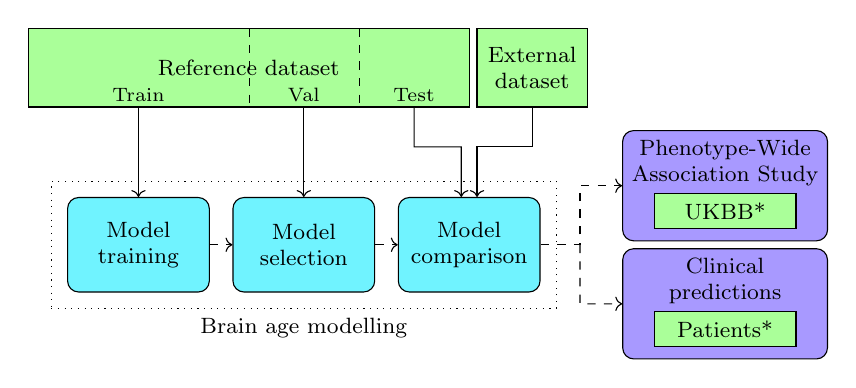
\begin{tikzpicture}[
			every node/.append style={font=\footnotesize}
		]
			\node[draw=black,minimum width=5.6cm,minimum height=1cm,fill=dataset] at (0.2,-1) {Reference dataset};
			\node[draw=none,minimum width=2.8cm,minimum height=1cm] (train) at (-1.2,-1.35) {\scriptsize{Train}};
			\node[draw=none,minimum width=1.4cm,minimum height=1cm] at (0.9,-1.35) (val) {\scriptsize{Val}};
			\node[draw=none,minimum width=1.4cm,minimum height=1cm] at (2.3,-1.35) (test) {\scriptsize{Test}};
			\node[draw=black,minimum height=1cm,minimum width=1.4cm,fill=dataset,align=center] (external) at (3.8,-1) {External\\dataset};
			\node[draw=black,rounded corners,align=center,minimum height=1.2cm, minimum width=1.8cm,fill=process] (training) at (-1.2,-3.25) {Model \\ training};
			\node[draw=black,rounded corners,align=center,minimum height=1.2cm, minimum width=1.8cm,fill=process] (selection) at (0.9,-3.25) {Model \\ selection};
			\node[draw=black,rounded corners,align=center,minimum height=1.2cm, minimum width=1.8cm,fill=process] (comparison) at (3,-3.25) {Model \\ comparison};
			\node[draw=black,rounded corners,align=center,minimum height=1.4cm, minimum width=2.6cm,fill=application, text depth=0.3cm] (pwas) at (6.25,-2.5) {Phenotype-Wide \\ Association Study \\};
			\node[draw=black,rounded corners,align=center,minimum height=1.4cm, minimum width=2.6cm,fill=application, text depth=0.3cm] (preds) at (6.25,-4) {Clinical \\ predictions \\};
			\node[draw=black,minimum height=0.4cm,minimum width=1.8cm,fill=dataset,align=center] at (6.25,-2.82) {UKBB*};
			\node[draw=black,minimum height=0.4cm,minimum width=1.8cm,fill=dataset,align=center] at (6.25,-4.32) {Patients*};
			\path[draw=black,->] ($ (train.south) + (0,0.35) $) -- (training) {};
			\path[draw=black,->] ($ (val.south) + (0,0.35) $) -- (selection) {};
			\path[draw=black,->] ($ (test.south) + (0,0.35) $) -- ($ (test.south) + (0,-0.15) $) -- ($ (test.south) + (0.6,-0.15) $) -- ($ (comparison.north) + (-0.1,0) $) {};
			\path[draw=black,->] (external.south) -- ($ (external.south) + (0,-0.5) $) -- ($ (external.south) + (-0.7,-0.5) $) -- ($ (comparison.north) + (0.1,0) $) {};
			\path[draw=black,->,dashed] (training) -- (selection) {};
			\path[draw=black,->,dashed] (selection) -- (comparison) {};
			\path[draw=black,->,dashed] (comparison.east) -- ($ (comparison.east) + (0.5,0) $) -- ($ (comparison.east) + (0.5,0.75) $) -- (pwas.west) {};
			\path[draw=black,->,dashed]($ (comparison.east) + (0.5,0) $) -- ($ (comparison.east) + (0.5,-0.75) $) -- (preds.west) {};
			\draw[dashed] ($ (train.east) + (0,0.85) $) -- ($ (train.east) + (0,-0.15) $) {};
			\draw[dashed] ($ (val.east) + (0,0.85) $) -- ($ (val.east) + (0,-0.15) $) {};

			\draw[dotted] ($ (training.south west) + (-0.2,-0.2) $) -- node[below] {Brain age modelling} ($ (comparison.south east) + (0.2,-0.2) $) -- ($ (comparison.north east) + (0.2,0.2) $) -- ($ (training.north west) + (-0.2,0.2) $) -- ($ (training.south west) + (-0.2,-0.2) $) {};
		\end{tikzpicture}
	\end{frame}

	\begin{frame}{Paper 1: Brain age} % Predictions
		\def\N{1}
		\centering
		\vfill
		\begin{tikzpicture}
			\begin{groupplot}[
				group style={
					group size=3 by 2,
					horizontal sep=0.4cm,
					vertical sep=0.8cm
				},
				width=0.4\linewidth,
				height=0.4\linewidth
			]

			  \nextgroupplot[
				  xmin=0,
				  xmax=100,
				  ymin=0,
				  ymax=100,
				  xtick pos=bottom,
				  ytick pos=left,
				  xticklabels={,,},
				  ticklabel style = {font=\footnotesize}
			  ]
				  \addplot [red] coordinates {(0,0) (100,100)};
				  \addplot [
					  only marks,
					  mark size=0.75pt,
					  color=black,
					  opacity=0.35
				  ] table [
					  x=classification,
					  y=age,
					  each nth point={\N},
					  col sep=comma
				  ] {data/paper1/prediction/test_predictions.csv};
				  \node [anchor=south east,inner sep=0pt,outer sep=0pt] (outofsample) at (rel axis cs:0.92,0.08) {\footnotesize{\textcolor{red}{MAE=2.23}}};
			  \nextgroupplot[
				  xmin=0,
				  xmax=100,
				  ymin=0,
				  ymax=100,
				  xtick pos=bottom,
				  ytick pos=left,
				  xticklabels={,,},
				  yticklabels={,,}
			  ]
				  \addplot [red] coordinates {(0,0) (100,100)};
				  \addplot [
					  only marks,
					  mark size=0.75pt,
					  color=black,
					  opacity=0.35
				  ] table [
					  x=regression,
					  y=age,
					  each nth point={\N},
					  col sep=comma
				  ] {data/paper1/prediction/test_predictions.csv};
				  \node [anchor=south east,inner sep=0pt,outer sep=0pt] (outofsample) at (rel axis cs:0.92,0.08) {\footnotesize{\textcolor{red}{MAE=2.47}}};

			  \nextgroupplot[
				  xmin=0,
				  xmax=100,
				  ymin=0,
				  ymax=100,
				  xtick pos=bottom,
				  ytick pos=left,
				  xticklabels={,,},
				  yticklabels={,,}
			  ]
				  \addplot [red] coordinates {(0,0) (100,100)};
				  \addplot [
					  only marks,
					  mark size=0.75pt,
					  color=black,
					  opacity=0.35
				  ] table [
					  x=ranking,
					  y=age,
					  each nth point={\N},
					  col sep=comma
				  ] {data/paper1/prediction/test_predictions.csv};
				  \node [anchor=south east,inner sep=0pt,outer sep=0pt] (outofsample) at (rel axis cs:0.92,0.08) {\footnotesize{\textcolor{red}{MAE=2.55}}};

			  \nextgroupplot[
				  xmin=0,
				  xmax=100,
				  ymin=0,
				  ymax=100,
				  xtick pos=bottom,
				  ytick pos=left,
				  ticklabel style = {font=\footnotesize}
			  ]
				  \addplot [red] coordinates {(0,0) (100,100)};
				  \addplot [
					  only marks,
					  mark size=0.75pt,
					  color=black,
					  opacity=0.35
				  ] table [
					  x=classification,
					  y=age,
					  each nth point={\N},
					  col sep=comma
				  ] {data/paper1/prediction/external_predictions.csv};
				  \node [anchor=south east,inner sep=0pt,outer sep=0pt] (outofsample) at (rel axis cs:0.92,0.08) {\footnotesize{\textcolor{red}{MAE=5.04}}};
			  \nextgroupplot[
				  xmin=0,
				  xmax=100,
				  ymin=0,
				  ymax=100,
				  xtick pos=bottom,
				  ytick pos=left,
				  yticklabels={,,},
				  ticklabel style = {font=\footnotesize}
			  ]
				  \addplot [red] coordinates {(0,0) (100,100)};
				  \addplot [
					  only marks,
					  mark size=0.75pt,
					  color=black,
					  opacity=0.35
				  ] table [
					  x=regression,
					  y=age,
					  each nth point={\N},
					  col sep=comma
				  ] {data/paper1/prediction/external_predictions.csv};
				  \node [anchor=south east,inner sep=0pt,outer sep=0pt] (outofsample) at (rel axis cs:0.92,0.08) {\footnotesize{\textcolor{red}{MAE=3.90}}};

			  \nextgroupplot[
				  xmin=0,
				  xmax=100,
				  ymin=0,
				  ymax=100,
				  xtick pos=bottom,
				  ytick pos=left,
				  yticklabels={,,},
				  ticklabel style = {font=\footnotesize}
			  ]
				  \addplot [red] coordinates {(0,0) (100,100)};
				  \addplot [
					  only marks,
					  mark size=0.75pt,
					  color=black,
					  opacity=0.35
				  ] table [
					  x=ranking,
					  y=age,
					  each nth point={\N},
					  col sep=comma
				  ] {data/paper1/prediction/external_predictions.csv};
				  \node [anchor=south east,inner sep=0pt,outer sep=0pt] (outofsample) at (rel axis cs:0.92,0.08) {\footnotesize{\textcolor{red}{MAE=5.92}}};
		  \end{groupplot}
		  \node [] at ($ (group c1r1.north) + (0,0.25) $) {Soft Classification};
		  \node [] at ($ (group c2r1.north) + (0,0.25) $) {Regression};
		  \node [] at ($ (group c3r1.north) + (0,0.25) $) {Ranking};
		  \node [rotate=90] (ylabel) at ($(group c1r1.west)!0.5!(group c1r2.west)+(-0.9,0cm)$) {\footnotesize{Chronological age}};
		  \node [] (xlabel) at ($(group c2r2.south)+(0,-0.7cm)$) {\footnotesize{Predicted brain age}};
		  \node (left) at ($(group c1r1.west)!0.5!(group c1r2.west) + (-0.3,0cm) $) {};
		  \node (right) at ($(group c3r1.east)!0.5!(group c3r2.east) + (0.3,0cm) $) {};
		  \path [draw=black,dotted](left) -- (right) {};
		  \node [anchor=south east,align=right,inner sep=1pt,outer sep=0pt] at ($(group c3r1.east)!0.5!(group c3r2.east) + (0.3,0cm) $) {\scriptsize{Test split}};
		  \node [anchor=north east,align=right,inner sep=1pt,outer sep=0pt] at ($(group c3r1.east)!0.5!(group c3r2.east) + (0.3,0cm) $) {\scriptsize{External dataset}};
	  \end{tikzpicture}
	  \vfill
	\end{frame}

	\begin{frame}{Paper 1: Brain age} % PheWAS
		\begin{tikzpicture}[scale=0.8]
			\begin{groupplot}[
				group style={
					  group size=1 by 2,
					  vertical sep=0.4cm
				  },
				  width=1.1\linewidth,
				  height=0.45\linewidth
			  ]
			  \nextgroupplot[
				width=1.05\textwidth,
				height=0.4\textwidth,
				xmin=-2,
				xmax=350,
				ymin=-9,
				ymax=0,
				xticklabels={,,},
				ytick={-2,-4,-6,-8},
				yticklabels={2, 4, 6, 8},
				axis x line*=bottom,
				axis y line=left,
				y axis line style={stealth-},
				y dir=reverse
			]
				\addplot [draw=black,fill=red!80,only marks,mark size=1.5pt] table [col sep=comma, x=idx,y expr=\thisrow{female} * -1] {data/paper1/phewas/pvalues.csv};\label{trace:female}
				\addplot [black,line width=0.5,dotted] coordinates {(65,-10) (65,10)};
				\addplot [black,line width=0.5,dotted] coordinates {(88,-10) (88,10)};
				\addplot [black,line width=0.5,dotted] coordinates {(150,-10) (150,10)};
				\addplot [black,line width=0.5,dotted] coordinates {(182,-10) (182,10)};
				\addplot [black,line width=0.5,dotted] coordinates {(205,-10) (205,10)};
				\addplot [black,line width=0.5,dotted] coordinates {(230,-10) (230,10)};
				\addplot [black,line width=0.5,dotted] coordinates {(247,-10) (247,10)};
				\addplot [black,line width=0.5,dotted] coordinates {(270,-10) (270,10)};
				\addplot [black,line width=0.5,dotted] coordinates {(289,-10) (289,10)};
				\addplot [black,line width=0.5,dotted] coordinates {(317,-10) (317,10)};
				\addplot [black,line width=0.5,dotted] coordinates {(324,-10) (324,10)};
				\addplot [black,line width=0.5,dotted] coordinates {(336,-10) (336,10)};
				\addplot [black,dashed] coordinates {(-10,-3.833) (400,-3.822)};
				\addplot [black,dashed] coordinates {(-10,-2.700) (400,-2.598)};
				\node [] at (axis cs:25,-4.78) {\scriptsize{IGF-1}};
				\node [] at (axis cs:113,-4.49) {\scriptsize{Diabetes diagnosis}};
				\node (dbpa) [circle,draw=none,inner sep=0pt,minimum size=2.4pt] at (axis cs:208,-4.38) {};
				\node (dbpatext) at (axis cs:125,-6.2) {\scriptsize{Diastolic blood pressure}};
				\path [draw=black,->] (dbpatext) -- (dbpa) {};
				\node (dbpm) [circle,draw=none,inner sep=0pt,minimum size=2.4pt] at (axis cs:209,-4.65) {};
				\node (dbpmtext) at (axis cs:202,-8.2) {\scriptsize{Diastolic blood pressure (manual)}};
				\path [draw=black,->] (dbpmtext) -- (dbpm) {};
				\node (sbpa) [circle,draw=none,inner sep=0pt,minimum size=2.4pt] at (axis cs:224,-4.56) {};
				\node (sbpatext) at (axis cs:280,-6.7) {\scriptsize{Systolic blood pressure}};
				\path [draw=black,->] (sbpatext) -- (sbpa) {};

			\nextgroupplot[
				width=1.05\textwidth,
				height=0.4\textwidth,
				xmin=-2,
				xmax=350,
				ymin=0,
				ymax=9,
				xticklabels={,,},
				ytick={0,2,4,6,8},
				axis x line*=top,
				axis y line=left,
				y dir=reverse
			]
				\addplot [draw=black,fill=blue!80,only marks,mark size=1.5pt] table [col sep=comma, x=idx,y=male] {data/paper1/phewas/pvalues.csv};\label{trace:male}
				\addplot [black,line width=0.5,dotted] coordinates {(65,-10) (65,10)};
				\addplot [black,line width=0.5,dotted] coordinates {(88,-10) (88,10)};
				\addplot [black,line width=0.5,dotted] coordinates {(150,-10) (150,10)};
				\addplot [black,line width=0.5,dotted] coordinates {(182,-10) (182,10)};
				\addplot [black,line width=0.5,dotted] coordinates {(205,-10) (205,10)};
				\addplot [black,line width=0.5,dotted] coordinates {(230,-10) (230,10)};
				\addplot [black,line width=0.5,dotted] coordinates {(247,-10) (247,10)};
				\addplot [black,line width=0.5,dotted] coordinates {(270,-10) (270,10)};
				\addplot [black,line width=0.5,dotted] coordinates {(289,-10) (289,10)};
				\addplot [black,line width=0.5,dotted] coordinates {(317,-10) (317,10)};
				\addplot [black,line width=0.5,dotted] coordinates {(324,-10) (324,10)};
				\addplot [black,line width=0.5,dotted] coordinates {(336,-10) (336,10)};
				\addplot [black,dashed] coordinates {(-10,3.822) (400,3.822)};
				\addplot [black,dashed] coordinates {(-10,2.598) (400,2.598)};
				\node [] at (axis cs:18,7.85) {\scriptsize{Glucose}};
				\node [] at (axis cs:25,6.53) {\scriptsize{IGF-1}};
				\node (mcv) [circle,draw=none,inner sep=0pt,minimum size=2.4pt] at (axis cs:33,4.85) {};
				\node (mcvtext) at (axis cs:80,8.6) {\scriptsize{Mean corpuscular volume}};
				\path [draw=black,->] (mcvtext) -- (mcv) {};
				\node (pc) [circle,draw=none,inner sep=0pt,minimum size=2.4pt] at (axis cs:47,4.50) {};
				\node (pctext) at (axis cs:100,6.4) {\scriptsize{Platelet crit}};
				\path [draw=black,->] (pctext) -- (pc) {};
				\node [] at (axis cs:113,4.43) {\scriptsize{Diabetes diagnosis}};
				\node (cereal) [circle,draw=none,inner sep=0pt,minimum size=2.4pt] at (axis cs:250,4.62) {};
				\node (cerealtext) [] at (axis cs:225,6.52) {\scriptsize{Cereal intake}};
				\path [draw=black,->] (cerealtext) -- (cereal) {};
				\node (beer) [circle,draw=none,inner sep=0pt,minimum size=2.4pt] at (axis cs:280,6.05) {};
				\node (beertext) [] at (axis cs:272,8) {\scriptsize{Average weekly beer plus cider intake}};
				\path [draw=black,->] (beertext) -- (beer) {};
				\node [] at (axis cs:291,5.23) {\scriptsize{Age stopped smoking}};


			\end{groupplot}

			\node [rotate=90] (ylabel) at ($(group c1r1.center)!0.5!(group c1r2.center)+(-6.25,0cm)$) {$-log_{10}(p)$};
			\node[draw=black] at ($ (group c1r2.center) + (0,-2cm) $) {\ref{trace:male} \footnotesize{Male} \ref{trace:female} \footnotesize{Female}};
			\end{tikzpicture}
	\end{frame}

	\begin{frame}{Paper 1: Brain age} % Disorders
		\begin{minipage}{0.4\textwidth}
			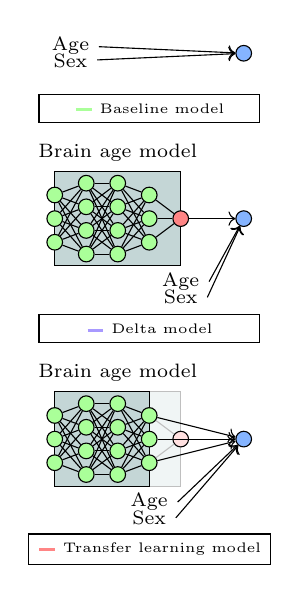
\begin{tikzpicture}
				\def\nodesize{2pt}
				\def\hsep{0.3}
				\def\vsep{0.4}
				\def\boxsize{2.8cm}

				\def\basey{9.6}
				\def\deltay{7.5}
				\def\transfery{4.7}
				\node [] (age) at (0.5 * \vsep, \basey + 0.1) {\scriptsize{Age}};
				\node [] (sex) at (0.5 * \vsep, \basey - 0.1) {\scriptsize{Sex}};
				\node [circle,draw=black,fill=prediction, inner sep=\nodesize] (pred) at (6 * \vsep,\basey) {};

				\path [->,draw=black] (age) -- (pred) {};
				\path [->,draw=black] (sex) -- (pred) {};
				\node [font=\tiny,draw=black,minimum width=\boxsize] at (3 * \vsep, \basey - 0.7) {\adjustbox{valign=c}{\tikz \draw[base, very thick] (0,0) -- (0.2,0);} Baseline model};

			\node [rectangle, draw=black,minimum height=1.2cm,minimum width=1.6cm,label=\scriptsize{Brain age model},fill=model] at (2 * \vsep,\deltay) {};
				\node [circle, draw=black,fill=nodes, inner sep=\nodesize] (00) at (0,\deltay - \hsep) {};
				\node [circle, draw=black,fill=nodes, inner sep=\nodesize] (01) at (0,\deltay) {};
				\node [circle, draw=black,fill=nodes, inner sep=\nodesize] (02) at (0,\deltay + \hsep) {};
				\node [circle, draw=black,fill=nodes, inner sep=\nodesize] (10) at (\vsep,\deltay - 1.5 * \hsep) {};
				\node [circle, draw=black,fill=nodes, inner sep=\nodesize] (11) at (\vsep,\deltay - 0.5 * \hsep) {};
				\node [circle, draw=black,fill=nodes, inner sep=\nodesize] (12) at (\vsep,\deltay + 0.5 * \hsep) {};
				\node [circle, draw=black,fill=nodes, inner sep=\nodesize] (13) at (\vsep,\deltay + 1.5 * \hsep) {};
				\node [circle, draw=black,fill=nodes, inner sep=\nodesize] (20) at (2 * \vsep,\deltay - 1.5 * \hsep) {};
				\node [circle, draw=black,fill=nodes, inner sep=\nodesize] (21) at (2 * \vsep,\deltay - 0.5 * \hsep) {};
				\node [circle, draw=black,fill=nodes, inner sep=\nodesize] (22) at (2 * \vsep,\deltay + 0.5 * \hsep) {};
				\node [circle, draw=black,fill=nodes, inner sep=\nodesize] (23) at (2 * \vsep,\deltay + 1.5 * \hsep) {};
				\node [circle, draw=black,fill=nodes, inner sep=\nodesize] (30) at (3 * \vsep,\deltay -  \hsep) {};
				\node [circle, draw=black,fill=nodes, inner sep=\nodesize] (31) at (3 * \vsep,\deltay) {};
				\node [circle, draw=black,fill=nodes, inner sep=\nodesize] (32) at (3 * \vsep,\deltay + \hsep) {};
				\node [circle, draw=black,fill=delta, inner sep=\nodesize] (40) at (4 * \vsep,\deltay) {};

				\node [draw=none] (age) at (4 * \vsep,\deltay - 0.8) {\scriptsize{Age}};
				\node [draw=none] (sex) at (4 * \vsep,\deltay - 1.0) {\scriptsize{Sex}};

				\node [circle,draw=black,fill=prediction, inner sep=\nodesize] (pred) at (6 * \vsep,\deltay) {};

				\path [-,draw=black] (00) -- (10) {};
				\path [-,draw=black] (00) -- (11) {};
				\path [-,draw=black] (00) -- (12) {};
				\path [-,draw=black] (00) -- (13) {};
				\path [-,draw=black] (01) -- (10) {};
				\path [-,draw=black] (01) -- (11) {};
				\path [-,draw=black] (01) -- (12) {};
				\path [-,draw=black] (01) -- (13) {};
				\path [-,draw=black] (02) -- (10) {};
				\path [-,draw=black] (02) -- (11) {};
				\path [-,draw=black] (02) -- (12) {};
				\path [-,draw=black] (02) -- (13) {};

				\path [-,draw=black] (10) -- (20) {};
				\path [-,draw=black] (10) -- (21) {};
				\path [-,draw=black] (10) -- (22) {};
				\path [-,draw=black] (10) -- (23) {};
				\path [-,draw=black] (11) -- (20) {};
				\path [-,draw=black] (11) -- (21) {};
				\path [-,draw=black] (11) -- (22) {};
				\path [-,draw=black] (11) -- (23) {};
				\path [-,draw=black] (12) -- (20) {};
				\path [-,draw=black] (12) -- (21) {};
				\path [-,draw=black] (12) -- (22) {};
				\path [-,draw=black] (12) -- (23) {};
				\path [-,draw=black] (13) -- (20) {};
				\path [-,draw=black] (13) -- (21) {};
				\path [-,draw=black] (13) -- (22) {};
				\path [-,draw=black] (13) -- (23) {};

				\path [-,draw=black] (20) -- (30) {};
				\path [-,draw=black] (20) -- (31) {};
				\path [-,draw=black] (20) -- (32) {};
				\path [-,draw=black] (21) -- (30) {};
				\path [-,draw=black] (21) -- (31) {};
				\path [-,draw=black] (21) -- (32) {};
				\path [-,draw=black] (22) -- (30) {};
				\path [-,draw=black] (22) -- (31) {};
				\path [-,draw=black] (22) -- (32) {};
				\path [-,draw=black] (23) -- (30) {};
				\path [-,draw=black] (23) -- (31) {};
				\path [-,draw=black] (23) -- (32) {};

				\path [-,draw=black] (30) -- (40) {};
				\path [-,draw=black] (31) -- (40) {};
				\path [-,draw=black] (32) -- (40) {};

				\path [-> ,draw=black] (40) -- (pred) {};
				\path [->,draw=black] (sex.east) -- (pred) {};
				\path [->,draw=black] (age.east) -- (pred) {};

				\node [font=\tiny,draw=black,minimum width=\boxsize] at (3 * \vsep, \deltay - 1.4) {\adjustbox{valign=c}{\tikz \draw[lasso, very thick] (0,0) -- (0.2,0);} Delta model};


				\node [rectangle, draw=black!25,minimum height=1.2cm,minimum width=1.6cm,label=\scriptsize{Brain age model},fill=model!25] at (2 * \vsep,\transfery) {};
				\node [rectangle, draw=black,minimum height=1.2cm,minimum width=1.2cm,fill=model] at (1.5 * \vsep, \transfery) {};
				\node [circle, draw=black,fill=nodes, inner sep=\nodesize] (00) at (0,\transfery - \hsep) {};
				\node [circle, draw=black,fill=nodes, inner sep=\nodesize] (01) at (0,\transfery) {};
				\node [circle, draw=black,fill=nodes, inner sep=\nodesize] (02) at (0,\transfery + \hsep) {};
				\node [circle, draw=black,fill=nodes, inner sep=\nodesize] (10) at (\vsep,\transfery - 1.5 * \hsep) {};
				\node [circle, draw=black,fill=nodes, inner sep=\nodesize] (11) at (\vsep,\transfery - 0.5 * \hsep) {};
				\node [circle, draw=black,fill=nodes, inner sep=\nodesize] (12) at (\vsep,\transfery + 0.5 * \hsep) {};
				\node [circle, draw=black,fill=nodes, inner sep=\nodesize] (13) at (\vsep,\transfery + 1.5 * \hsep) {};
				\node [circle, draw=black,fill=nodes, inner sep=\nodesize] (20) at (2 * \vsep,\transfery - 1.5 * \hsep) {};
				\node [circle, draw=black,fill=nodes, inner sep=\nodesize] (21)  at (2 * \vsep,\transfery - 0.5 * \hsep) {};
				\node [circle, draw=black,fill=nodes, inner sep=\nodesize] (22)  at (2 * \vsep,\transfery + 0.5 * \hsep) {};
				\node [circle, draw=black,fill=nodes, inner sep=\nodesize] (23)  at (2 * \vsep,\transfery + 1.5 * \hsep) {};
				\node [circle, draw=black,fill=nodes, inner sep=\nodesize] (30)  at (3 * \vsep,\transfery - \hsep) {};
				\node [circle, draw=black,fill=nodes, inner sep=\nodesize] (31)  at (3 * \vsep,\transfery) {};
				\node [circle, draw=black,fill=nodes, inner sep=\nodesize] (32)  at (3 * \vsep,\transfery + \hsep) {};
				\node [circle, draw=black,fill=delta!25, inner sep=\nodesize] (40)  at (4 * \vsep,\transfery) {};

				\node [draw=none] (age) at (3 * \vsep, \transfery - 0.8) {\scriptsize{Age}};
				\node [draw=none] (sex) at (3 * \vsep, \transfery - 1.0) {\scriptsize{Sex}};

				\node [circle,draw=black,fill=prediction, inner sep=\nodesize] (pred) at (6 * \vsep,\transfery) {};

				\path [-,draw=black] (00) -- (10) {};
				\path [-,draw=black] (00) -- (11) {};
				\path [-,draw=black] (00) -- (12) {};
				\path [-,draw=black] (00) -- (13) {};
				\path [-,draw=black] (01) -- (10) {};
				\path [-,draw=black] (01) -- (11) {};
				\path [-,draw=black] (01) -- (12) {};
				\path [-,draw=black] (01) -- (13) {};
				\path [-,draw=black] (02) -- (10) {};
				\path [-,draw=black] (02) -- (11) {};
				\path [-,draw=black] (02) -- (12) {};
				\path [-,draw=black] (02) -- (13) {};

				\path [-,draw=black] (10) -- (20) {};
				\path [-,draw=black] (10) -- (21) {};
				\path [-,draw=black] (10) -- (22) {};
				\path [-,draw=black] (10) -- (23) {};
				\path [-,draw=black] (11) -- (20) {};
				\path [-,draw=black] (11) -- (21) {};
				\path [-,draw=black] (11) -- (22) {};
				\path [-,draw=black] (11) -- (23) {};
				\path [-,draw=black] (12) -- (20) {};
				\path [-,draw=black] (12) -- (21) {};
				\path [-,draw=black] (12) -- (22) {};
				\path [-,draw=black] (12) -- (23) {};
				\path [-,draw=black] (13) -- (20) {};
				\path [-,draw=black] (13) -- (21) {};
				\path [-,draw=black] (13) -- (22) {};
				\path [-,draw=black] (13) -- (23) {};

				\path [-,draw=black] (20) -- (30) {};
				\path [-,draw=black] (20) -- (31) {};
				\path [-,draw=black] (20) -- (32) {};
				\path [-,draw=black] (21) -- (30) {};
				\path [-,draw=black] (21) -- (31) {};
				\path [-,draw=black] (21) -- (32) {};
				\path [-,draw=black] (22) -- (30) {};
				\path [-,draw=black] (22) -- (31) {};
				\path [-,draw=black] (22) -- (32) {};
				\path [-,draw=black] (23) -- (30) {};
				\path [-,draw=black] (23) -- (31) {};
				\path [-,draw=black] (23) -- (32) {};

				\path [-,draw=black!25] (30) -- (40) {};
				\path [-,draw=black!25] (31) -- (40) {};
				\path [-,draw=black!25] (32) -- (40) {};

				\path [-> ,draw=black] (30) -- (pred) {};
				\path [-> ,draw=black] (31) -- (pred) {};
				\path [-> ,draw=black] (32) -- (pred) {};
				\path [->,draw=black] (sex.east) -- (pred) {};
				\path [->,draw=black] (age.east) -- (pred) {};

				\node [font=\tiny,draw=black,minimum width=\boxsize] at (3 * \vsep, \transfery - 1.4) {\adjustbox{valign=c}{\tikz \draw[features, very thick] (0,0) -- (0.2,0);} Transfer learning model};
			\end{tikzpicture}
		\end{minipage}
		\begin{minipage}{0.59\textwidth}
			\begin{tikzpicture}
				\newcommand \ymin {-1.2}
				\newcommand \ymax {1.2}

				\begin{groupplot}[
					group style={
						group size=3 by 3,
						horizontal sep=0.25cm,
						vertical sep=0.25cm
					},
					height=0.55\textwidth,
					width=0.55\textwidth
				]
					\nextgroupplot[
						xmin=0,
						xmax=1,
						ymin=0,
						ymax=1,
						xticklabels={,,},
						yticklabels={,,},
						ticks=none
					]

					\addplot [black] coordinates {(0,0) (1,1)};
					\addplot [base,very thick] table [x=fpr,y=tpr] {\MSbaselineroc};\label{trace:baseline}
					\addplot [lasso,very thick] table [x=fpr,y=tpr] {\MSdeltaroc};\label{trace:delta}
					\addplot [features,very thick] table [x=fpr,y=tpr] {\MSfeaturesroc};\label{trace:features}

					\coordinate (MS) at (axis cs:1,0) {};

					\node [anchor=north west] at (axis cs: 0,1) {\textbf{\footnotesize{MS}}};

					\nextgroupplot[
						xmin=0,
						xmax=1,
						ymin=0,
						ymax=1,
						xticklabels={,,},
						yticklabels={,,},
						ticks=none
					]

					\addplot [black] coordinates {(0,0) (1,1)};
					\addplot [base,very thick] table [x=fpr,y=tpr] {\ADbaselineroc};
					\addplot [lasso,very thick] table [x=fpr,y=tpr] {\ADdeltaroc};
					\addplot [features,very thick] table [x=fpr,y=tpr] {\ADfeaturesroc};

					\coordinate (AD) at (axis cs:1,0) {};

					\node [anchor=north west] at (axis cs: 0,1) {\textbf{\footnotesize{AD}}};

					\nextgroupplot[
						xmin=0,
						xmax=1,
						ymin=0,
						ymax=1,
						xticklabels={,,},
						yticklabels={,,},
						ticks=none
					]

					\addplot [black] coordinates {(0,0) (1,1)};
					\addplot [base,very thick] table [x=fpr,y=tpr] {\MCIbaselineroc};
					\addplot [lasso,very thick] table [x=fpr,y=tpr] {\MCIdeltaroc};
					\addplot [features,very thick] table [x=fpr,y=tpr] {\MCIfeaturesroc};

					\coordinate (MCI) at (axis cs:1,0) {};

					\node [anchor=north west] at (axis cs: 0,1) {\textbf{\footnotesize{MCI}}};

					\nextgroupplot[
						xmin=0,
						xmax=1,
						ymin=0,
						ymax=1,
						xticklabels={,,},
						yticklabels={,,},
						ticks=none
					]

					\addplot [black] coordinates {(0,0) (1,1)};
					\addplot [base,very thick] table [x=fpr,y=tpr] {\SCZbaselineroc};
					\addplot [lasso,very thick] table [x=fpr,y=tpr] {\SCZdeltaroc};
					\addplot [features,very thick] table [x=fpr,y=tpr] {\SCZfeaturesroc};

					\coordinate (SCZ) at (axis cs:1,0) {};

					\node [anchor=north west] at (axis cs: 0,1) {\textbf{\footnotesize{SCZ}}};

					\nextgroupplot[
						xmin=0,
						xmax=1,
						ymin=0,
						ymax=1,
						xticklabels={,,},
						yticklabels={,,},
						ticks=none
					]

					\addplot [black] coordinates {(0,0) (1,1)};
					\addplot [base,very thick] table [x=fpr,y=tpr] {\PSYbaselineroc};
					\addplot [lasso,very thick] table [x=fpr,y=tpr] {\PSYdeltaroc};
					\addplot [features,very thick] table [x=fpr,y=tpr] {\PSYfeaturesroc};

					\coordinate (PSY) at (axis cs:1,0) {};

					\node [anchor=north west] at (axis cs: 0,1) {\textbf{\footnotesize{PSY}}};

					\nextgroupplot[
						xmin=0,
						xmax=1,
						ymin=0,
						ymax=1,
						xticklabels={,,},
						yticklabels={,,},
						ticks=none
					]

					\addplot [black] coordinates {(0,0) (1,1)};
					\addplot [base,very thick] table [x=fpr,y=tpr] {\MOODbaselineroc};
					\addplot [lasso,very thick] table [x=fpr,y=tpr] {\MOODdeltaroc};
					\addplot [features,very thick] table [x=fpr,y=tpr] {\MOODfeaturesroc};

					\coordinate (MOOD) at (axis cs:1,0) {};

					\node [anchor=north west] at (axis cs: 0,1) {\textbf{\footnotesize{MOOD}}};

				\end{groupplot}

				\matrix [
					matrix of nodes,
					draw=none,
					row sep=-0.15cm,
					column sep=-0.2cm,
					anchor=south east,
					column 2/.style={nodes={font=\tiny}},
					outer sep=-2pt,
					ampersand replacement=\&
				] at (MS) {
					\&\underline{AUC}\\
					\adjustbox{valign=c}{\tikz \draw[base, very thick] (0,0) -- (0.2,0);}\&0.50\\
					\adjustbox{valign=c}{\tikz \draw[lasso, very thick] (0,0) -- (0.2,0);}\&0.71\\
					\adjustbox{valign=c}{\tikz \draw[features, very thick] (0,0) -- (0.2,0);}\&0.79\\
				};

				\matrix [
					matrix of nodes,
					draw=none,
					row sep=-0.15cm,
					column sep=-0.2cm,
					anchor=south east,
					column 2/.style={nodes={font=\tiny}},
					outer sep=-2pt,
					ampersand replacement=\&
				] at (AD) {
					\&\underline{AUC}\\
					\adjustbox{valign=c}{\tikz \draw[base, very thick] (0,0) -- (0.2,0);}\&0.51\\
					\adjustbox{valign=c}{\tikz \draw[lasso, very thick] (0,0) -- (0.2,0);}\&0.69\\
					\adjustbox{valign=c}{\tikz \draw[features, very thick] (0,0) -- (0.2,0);}\&0.83\\
				};

				\matrix [
					matrix of nodes,
					draw=none,
					row sep=-0.15cm,
					column sep=-0.2cm,
					anchor=south east,
					column 2/.style={nodes={font=\tiny}},
					outer sep=-2pt,
					ampersand replacement=\&
				] at (MCI) {
					\&\underline{AUC}\\
					\adjustbox{valign=c}{\tikz \draw[base, very thick] (0,0) -- (0.2,0);}\&0.54\\
					\adjustbox{valign=c}{\tikz \draw[lasso, very thick] (0,0) -- (0.2,0);}\&0.65\\
					\adjustbox{valign=c}{\tikz \draw[features, very thick] (0,0) -- (0.2,0);}\&0.73\\
				};

				\matrix [
					matrix of nodes,
					draw=none,
					row sep=-0.15cm,
					column sep=-0.2cm,
					anchor=south east,
					column 2/.style={nodes={font=\tiny}},
					outer sep=-2pt,
					ampersand replacement=\&
				] at (SCZ) {
					\&\underline{AUC}\\
					\adjustbox{valign=c}{\tikz \draw[base, very thick] (0,0) -- (0.2,0);}\&0.50\\
					\adjustbox{valign=c}{\tikz \draw[lasso, very thick] (0,0) -- (0.2,0);}\&0.58\\
					\adjustbox{valign=c}{\tikz \draw[features, very thick] (0,0) -- (0.2,0);}\&0.62\\
				};

				\matrix [
					matrix of nodes,
					draw=none,
					row sep=-0.15cm,
					column sep=-0.2cm,
					anchor=south east,
					column 2/.style={nodes={font=\tiny}},
					outer sep=-2pt,
					ampersand replacement=\&
				] at (PSY) {
					\&\underline{AUC}\\
					\adjustbox{valign=c}{\tikz \draw[base, very thick] (0,0) -- (0.2,0);}\&0.47\\
					\adjustbox{valign=c}{\tikz \draw[lasso, very thick] (0,0) -- (0.2,0);}\&0.52\\
					\adjustbox{valign=c}{\tikz \draw[features, very thick] (0,0) -- (0.2,0);}\&0.62\\
				};

				\matrix [
					matrix of nodes,
					draw=none,
					row sep=-0.15cm,
					column sep=-0.2cm,
					anchor=south east,
					column 2/.style={nodes={font=\tiny}},
					outer sep=-2pt,
					ampersand replacement=\&
				] at (MOOD) {
					\&\underline{AUC}\\
					\adjustbox{valign=c}{\tikz \draw[base, very thick] (0,0) -- (0.2,0);}\&0.52\\
					\adjustbox{valign=c}{\tikz \draw[lasso, very thick] (0,0) -- (0.2,0);}\&0.55\\
					\adjustbox{valign=c}{\tikz \draw[features, very thick] (0,0) -- (0.2,0);}\&0.59\\
				};

			\end{tikzpicture}
		\end{minipage}
	\end{frame}

	\begin{frame}{Paper 2: Genetic architecture of brain age}
		\centering
		\vfill
		\begin{tikzpicture}
			\node[inner sep=1pt, fill=white, draw=black] {
				\includegraphics[width=8cm]{data/paper2.png}
			};
		\end{tikzpicture}
		\vfill
	\end{frame}

	\begin{frame}{Paper 2: Genetic architecture of brain age}
		\centering
		\vfill
		\begin{tikzpicture}
			\node[inner sep=1pt, fill=white, draw=black] {
				\includegraphics[width=10cm]{data/gwas.png}
			};
		\end{tikzpicture}
		\vfill
	\end{frame}

	\begin{frame}{Paper 2: Genetic architecture of brain age}
		\centering
		\vfill
		\begin{tikzpicture}
			\node[inner sep=1pt, fill=white, draw=black] {
				\includegraphics[width=8cm]{data/expression.png}
			};
		\end{tikzpicture}
		\vfill
	\end{frame}

	\begin{frame}{Paper 2: Genetic architecture of brain age}
		\centering
		\vfill
		\begin{tikzpicture}
			\node[inner sep=1pt, fill=white, draw=black] {
				\includegraphics[width=10.5cm]{data/correlation.png}
			};
		\end{tikzpicture}
		\vfill
	\end{frame}

	\begin{frame}{Paper 2: Genetic architecture of brain age}
		\centering
		\vfill
		\begin{tikzpicture}
			\node[inner sep=1pt, fill=white, draw=black] {
				\includegraphics[width=10.5cm]{data/causality.png}
			};
		\end{tikzpicture}
		\vfill
	\end{frame}

	\begin{frame}{Paper 3: Explainable AI and dementia} % Frontpage
		\centering
		\vfill
		\begin{tikzpicture}
			\node[inner sep=1pt, fill=white, draw=black] {
				\includegraphics[width=8cm]{data/paper3.png}
			};
		\end{tikzpicture}
		\vfill
	\end{frame}

	\begin{frame}{Paper 3: Explainable AI and dementia} % Dataset
		\pgfplotstableread[col sep=comma]{data/dementia_dataset/dementia_full.csv}\dementiafull
		\pgfplotstableread[col sep=comma]{data/dementia_dataset/dementia_addneuromed_GE_MEDICAL_SYSTEMS.csv}\dementiage
		\pgfplotstableread[col sep=comma]{data/dementia_dataset/dementia_addneuromed_PICKER_International_Inc.csv}\dementiapicker
		\pgfplotstableread[col sep=comma]{data/dementia_dataset/dementia_ADNI_15T.csv}\dementiaadnione
		\pgfplotstableread[col sep=comma]{data/dementia_dataset/dementia_ADNI_30T.csv}\dementiaadnithree
		\pgfplotstableread[col sep=comma]{data/dementia_dataset/dementia_AIBL_10.csv}\dementiaaiblone
		\pgfplotstableread[col sep=comma]{data/dementia_dataset/dementia_AIBL_20.csv}\dementiaaibltwo
		\pgfplotstableread[col sep=comma]{data/dementia_dataset/dementia_miriad_15_T_Signa.csv}\dementiamiriad
		\pgfplotstableread[col sep=comma]{data/dementia_dataset/dementia_oasis3_15T.csv}\dementiaoasisone
		\pgfplotstableread[col sep=comma]{data/dementia_dataset/dementia_oasis3_30T.csv}\dementiaoasisthree
		\pgfplotstableread[col sep=comma]{data/dementia_dataset/dementia_Oslo_GE750.csv}\dementiaoslo
		\pgfplotstableread[col sep=comma]{data/dementia_dataset/dementia_timepoints.csv}\dementiatimepoints

		\def\xmin{46}
		\def\xmax{99}
		\def\ymin{-1.4}
		\def\ymax{1.2}

		\centering
		\vfill
		\begin{tikzpicture}
            \begin{axis}[
                width=\textwidth,
                height=0.45\textwidth,
                xmin=\xmin,
                xmax=\xmax,
                ymin=-1.6,
                ymax=\ymax,
                xtick={55,60,65,70,75,80,85,90,95},
				axis lines=center,
				axis y line=none,
				clip=false
            ]
                \addplot[name path=zero, draw=none] coordinates {(47,0) (97,0)};
                \addplot[name path=fcases, draw=cases-default, very thick] table [x=x, y=F-cases]{\dementiafull};\label{trace:cases}
                \addplot[fill=cases-default, opacity=0.2] fill between [of=zero and fcases];
                \addplot[name path=fcontrols, draw=controls-default, very thick] table [x=x, y=F-controls]{\dementiafull};\label{trace:controls}
                \addplot[fill=controls-default, opacity=0.2] fill between [of=zero and fcontrols];
                \addplot[name path=mcases, draw=cases-default, very thick] table [x=x,y expr=\thisrow{M-cases} * -1]{\dementiafull};
                \addplot[fill=cases-default, opacity=0.2] fill between [of=zero and mcases];
                \addplot[name path=mcontrols, draw=controls-default, very thick] table [x=x,y expr=\thisrow{M-controls} * -1]{\dementiafull};
                \addplot[fill=controls-default, opacity=0.2] fill between [of=zero and mcontrols];
                \node[anchor=south west] at (axis cs: 46, 0.07) {\textbf{FEMALE}};
                \node[anchor=north west] at (axis cs: 46, -0.07) {\textbf{MALE}};
                \node[anchor=south, align=center] (n) at (axis cs: 72.5,-1.6) {n=1708};
                \node[anchor=north,font=\footnotesize] at ($(n.south) + (0,-2.5) $) {\ref{trace:controls} Controls\hspace{0.3cm}\ref{trace:cases} Cases};
            \end{axis}
        \end{tikzpicture}
		\vspace{-0.1cm}

			\newcommand{\scannersubplot}[3]{
				\nextgroupplot[
						axis lines=center,
						axis y line=none,
						xmin=\xmin,
						xmax=\xmax,
						ymin=\ymin - 0.25,
						ymax=\ymax + 0.25,
						xmajorticks=false,
						axis line style={-}
					]

						\addplot[name path=zero, draw=none] coordinates {(\xmin,0) (\xmax,0)};
						\addplot[name path=fcases, draw=cases-default, very thick] table [x=x, y=F-cases]{####1};
						\addplot[fill=cases-default, opacity=0.2] fill between [of=zero and fcases];
						\addplot[name path=fcontrols, draw=controls-default, very thick] table [x=x, y=F-controls]{####1};
						\addplot[fill=controls-default, opacity=0.2] fill between [of=zero and fcontrols];
						\addplot[name path=mcases, draw=cases-default, very thick] table [x=x,y expr=\thisrow{M-cases} * -1]{####1};
						\addplot[fill=cases-default, opacity=0.2] fill between [of=zero and mcases];
						\addplot[name path=mcontrols, draw=controls-default, very thick] table [x=x,y expr=\thisrow{M-controls} * -1]{####1};
						\addplot[fill=controls-default, opacity=0.2] fill between [of=zero and mcontrols];
						\node[anchor=south] at (axis cs: 72.5,1) {\tiny{####2}};
						\node[anchor=north] at (axis cs: 72.5,-1) {\tiny{\textbf{n=####3}}};
			}
			\begin{tikzpicture}
				\begin{groupplot}[
					group style={
						group size=5 by 2,
						horizontal sep=0.25cm,
						vertical sep=0.25cm
					},
					height=0.314\textwidth,
					width=0.314\textwidth
				]
					\scannersubplot{\dementiaadnithree}{ADNI 3.0T}{506}
					\scannersubplot{\dementiaoasisthree}{OASIS3 3.0T}{438}
					\scannersubplot{\dementiaadnione}{ADNI 1.5T}{290}
					\scannersubplot{\dementiaoslo}{Oslo GE750}{226}
					\scannersubplot{\dementiaaiblone}{AIBL Site 1}{92}
					\scannersubplot{\dementiage}{ANM GE}{74}
					\scannersubplot{\dementiamiriad}{MIRIAD}{38}
					\scannersubplot{\dementiaaibltwo}{AIBL Site 2}{22}
					\scannersubplot{\dementiapicker}{ANM Picker}{12}
					\scannersubplot{\dementiaoasisone}{OASIS3 1.5T}{10}
				\end{groupplot}
		\end{tikzpicture}

		\vfill
	\end{frame}

	\begin{frame}{Paper 3: Explainable AI and dementia} % Predictive performance
		\pgfplotstableread[col sep=comma]{data/test_distributions.csv}\testdistributions
		\pgfplotstableread[col sep=comma]{data/test_predictions.csv}\testpredictions

		\newcommand{\ymin}{-0.35}
		\newcommand{\ymax}{1.05}

		\begin{tikzpicture}
			\begin{axis}[
				name=distributions,
				height=0.4\textwidth,
				width=0.94\textwidth,
				xtick pos=bottom,
				ymajorticks=false,
				xmin=0,
				xmax=1,
				ymin=\ymin,
				ymax=\ymax,
				xlabel=\small{Prediction},
				every tick label/.append style={font=\footnotesize}
			]
				\addplot[name path=controls, draw=controls-default, very thick] table [x=prediction,y=controls]{\testdistributions};
				\addplot[name path=cases, draw=cases-default, very thick] table [x=prediction,y=cases]{\testdistributions};
				\addplot[name path=zero, draw=black] coordinates {(0,0) (1,0)};
				\addplot[fill=controls-default, opacity=0.2] fill between [of=zero and controls];
				\addplot[fill=cases-default, opacity=0.2] fill between [of=zero and cases];
				\addplot[
					scatter/classes={
						control={controls-default, draw=black, opacity=0.5},
						case={cases-default, draw=black, opacity=0.5}
					},
					scatter,
					mark=*,
					only marks,
					point meta=explicit symbolic
				] table [
					y expr=\thisrow{y} * -0.15 - 0.1,
					meta=class,
				] {\testpredictions};
				\addplot[dashed] coordinates {(0.5, \ymin) (0.5, \ymax)};
			\end{axis}
			% ONLY FOR ALIGNMENT
			\node[anchor=south east] at ($ (distributions.south west) + (0,0.28) $) {\textcolor{white}{\tiny{Controls}}};
			\node[anchor=south east] at ($ (distributions.south west) + (0,0.0) $) {\textcolor{white}{\tiny{Cases}}};

			\node[anchor=south west] at ($ (distributions.south east) + (0,0.28) $) {\tiny{Controls}};
			\node[anchor=south west] at ($ (distributions.south east) + (0,0.0) $) {\tiny{Cases}};
			\node[anchor=south,align=center] at (distributions.north) {\tiny{$t=0.5$}};
		\end{tikzpicture}

	\end{frame}

	\begin{frame}{Paper 3: Explainable AI and dementia} % Example relevance maps
		\centering
		\vfill
		\begin{tikzpicture}
			\node[
				minimum height=0.41\textwidth,
				minimum width=0.32\textwidth,
				fill=black
			] (box1) at (0, 0) {};
			\node[anchor=south] at (box1.south) {
				\includegraphics[width=0.31\textwidth]{data/subject1.png}
			};
			\node[anchor=north,inner sep=2pt, text=white, font=\footnotesize] at (box1.north) {Patient 1};

			\node
				[minimum height=0.41\textwidth,
				minimum width=0.32\textwidth,
				fill=black,
				anchor=west
			] (box2) at ($ (box1.east) + (0.05,0) $) {};
			\node[anchor=south] at (box2.south) {
				\includegraphics[width=0.31\textwidth]{data/subject2.png}
			};
			\node[anchor=north,inner sep=3pt, text=white, font=\footnotesize] at (box2.north) {Partient 2};

			\node
				[minimum height=0.41\textwidth,
				minimum width=0.32\textwidth,
				fill=black,
				anchor=west
			] (box3) at ($ (box2.east) + (0.05,0) $) {};
			\node[anchor=south] at (box3.south) {
				\includegraphics[width=0.31\textwidth]{data/subject3.png}
			};
			\node[anchor=north,inner sep=3pt, text=white, font=\footnotesize] at (box3.north) {Patient 3};

		\end{tikzpicture}
		\vfill
	\end{frame}

	\begin{frame}{Paper 3: Explainable AI and dementia} % Average maps
		\centering
		\vfill
		\begin{tikzpicture}
			\node[draw=none] at (-2, -2) {};
			\node[draw=none] at (6.5, 2.5) {};
			\node[label={[text depth=0]above:LRP}] at (0, 0) {
				\includegraphics[width=0.31\textwidth]{data/dementia.png}
			};
		\end{tikzpicture}
		\vfill
	\end{frame}

	\begin{frame}{Paper 3: Explainable AI and dementia} % Average maps
		\centering
		\vfill
		\begin{tikzpicture}
			\node[draw=none] at (-2, -2) {};
			\node[draw=none] at (6.5, 2.5) {};
			\node[label={[text depth=0]above:LRP}] at (0, 0) {
				\includegraphics[width=0.31\textwidth]{data/dementia.png}
			};

			\node[label={[text depth=0]above:GingerALE}] at (4.5, 0) {
				\includegraphics[width=0.31\textwidth]{data/ALE.png}
			};
		\end{tikzpicture}
		\vfill
	\end{frame}

	\begin{frame}{Paper 3: Explainable AI and dementia} % Overlap
		\centering
		\vfill
		\begin{tikzpicture}
            \node[
                minimum height=0.45\textwidth,
                minimum width=0.33\textwidth,
                fill=black
            ] (box1) at (0, 0) {};
            \node[anchor=south] at ($ (box1.south) + (0, 0.3) $) {
                \includegraphics[width=0.31\textwidth]{data/test_50.png}
            };
            \node[anchor=north,inner sep=2pt, text=white, font=\footnotesize] at (box1.north) {50th percentile};

            \node
                [minimum height=0.45\textwidth,
                minimum width=0.33\textwidth,
                fill=black,
                anchor=west
            ] (box2) at ($ (box1.east) + (0.05,0) $) {};
            \node[anchor=south] at ($ (box2.south) + (0, 0.3) $) {
                \includegraphics[width=0.31\textwidth]{data/test_70.png}
            };
            \node[anchor=north,inner sep=3pt, text=white, font=\footnotesize] at (box2.north) {70th percentile};

            \node
                [minimum height=0.45\textwidth,
                minimum width=0.33\textwidth,
                fill=black,
                anchor=west
            ] (box3) at ($ (box2.east) + (0.05,0) $) {};
            \node[anchor=south] at ($ (box3.south) + (0, 0.3) $) {
                \includegraphics[width=0.31\textwidth]{data/test_90.png}
            };
            \node[anchor=north,inner sep=3pt, text=white, font=\footnotesize] at (box3.north) {90th percentile};

            \node[anchor=south, inner sep=0pt, text depth=0] (overlap) at ($ (box2.south) + (0.1, 0.15) $) {\textcolor{white}{\scriptsize{Overlap}}};
            \node[anchor=east, inner sep=2pt, fill=yellow] (overlap-box) at ($ (overlap.west) + (-0.07, 0) $) {};
            \node[anchor=east, inner sep=0pt,text depth=0] (lrp) at ($ (overlap-box.west) + (-0.2, 0) $) {\textcolor{white}{\scriptsize{LRP}}};
            \node[anchor=east, inner sep=2pt, fill=green] at ($ (lrp.west) + (-0.07, 0) $) {};
            \node[anchor=west, inner sep=2pt, fill=red] (ale-box) at ($ (overlap.east) + (0.2, 0) $) {};
            \node[anchor=west, inner sep=0pt, text depth=0] at ($ (ale-box.east) + (0.07, 0) $) {\textcolor{white}{\scriptsize{ALE}}};

        \end{tikzpicture}
		\vfill
	\end{frame}

	\begin{frame}{Paper 3: Explainable AI and dementia} % Components
		\centering
		\vfill
		\begin{tikzpicture}
			\newcommand{\drawmask}[3]{
				\node[anchor=west] (second) at (####2*0.89, ####3*-1) {
					\includegraphics[
						width=0.9cm,
						clip=true,
						trim = 192mm 232mm 0mm 0mm
					]{data/components/component_####1.png}
				};
			}
			\foreach \i in {0,...,7}{
				\foreach \j in {0,...,7}{
					\pgfmathsetmacro{\idx}{int(\i * 8 + \j)}
					\drawmask{\idx}{\j}{\i}
				}
			}
		\end{tikzpicture}
		\vfill
	\end{frame}

	\begin{frame}{Paper 3: Explainable AI and dementia} % Prognosis
		\centering
		\vfill
		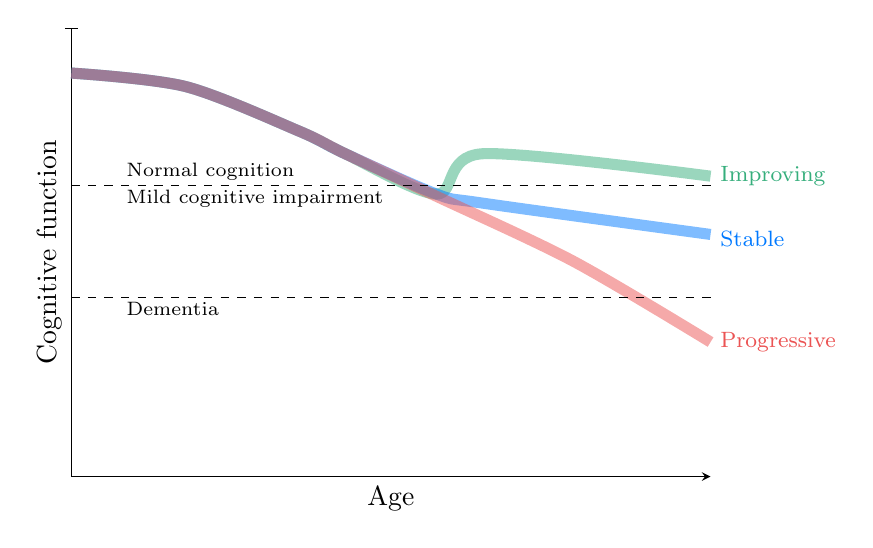
\begin{tikzpicture}
			\begin{axis}[
				height=0.6\textwidth,
				width=0.8\textwidth,
				xlabel={Age},
				ylabel={Cognitive function},
				ticks=none,
				axis x line=bottom,
				axis y line=left,
				y axis line style={-|},
				xmin=0,
				xmax=1.4,
				ymin=0,
				ymax=1,
				clip=false
			]
			\addplot[draw=healthy-default, smooth, line width=4pt, opacity=0.5] coordinates {
				(0, 0.9)
				(0.25, 0.87)
				(0.5, 0.77)
				(0.6, 0.72)
				(0.8, 0.63)
				(0.9, 0.72)
				(1.4, 0.67)
			};
			\addplot[draw=controls-default, smooth, line width=4pt, opacity=0.5] coordinates {
				(0, 0.9)
				(0.25, 0.87)
				(0.5, 0.77)
				(0.6, 0.72)
				(0.8, 0.63)
				(0.9, 0.61)
				(1.4, 0.54)
			};
			\addplot[draw=cases-default, smooth, line width=4pt, opacity=0.5] coordinates {
				(0, 0.9)
				(0.25, 0.87)
				(0.5, 0.77)
				(0.6, 0.72)
				(0.8, 0.625)
				(1.1, 0.48)
				(1.4, 0.3)
			};
			\addplot[dashed] coordinates {
				(0, 0.65)
				(1.4, 0.65)
			};
			\addplot[dashed] coordinates {
				(0, 0.4)
				(1.4, 0.4)
			};
			\node[anchor=south west] at (axis cs: 0.1, 0.64) {\scriptsize{Normal cognition}};
			\node[anchor=north west] at (axis cs: 0.1, 0.66) {\scriptsize{Mild cognitive impairment}};
			\node[anchor=north west] at (axis cs: 0.1, 0.41) {\scriptsize{Dementia}};
			\node[anchor=west] at (axis cs: 1.4, 0.67) {\textcolor{healthy-default}{\footnotesize{Improving}}};
			\node[anchor=west] at (axis cs: 1.4, 0.53) {\textcolor{controls-default}{\footnotesize{Stable}}};
			\node[anchor=west] at (axis cs: 1.4, 0.3) {\textcolor{cases-default}{\footnotesize{Progressive}}};
			\end{axis}
		\end{tikzpicture}
		\vfill
	\end{frame}

	\begin{frame}{Paper 3: Explainable AI and dementia} % Prognosis
		\centering
		\vfill
		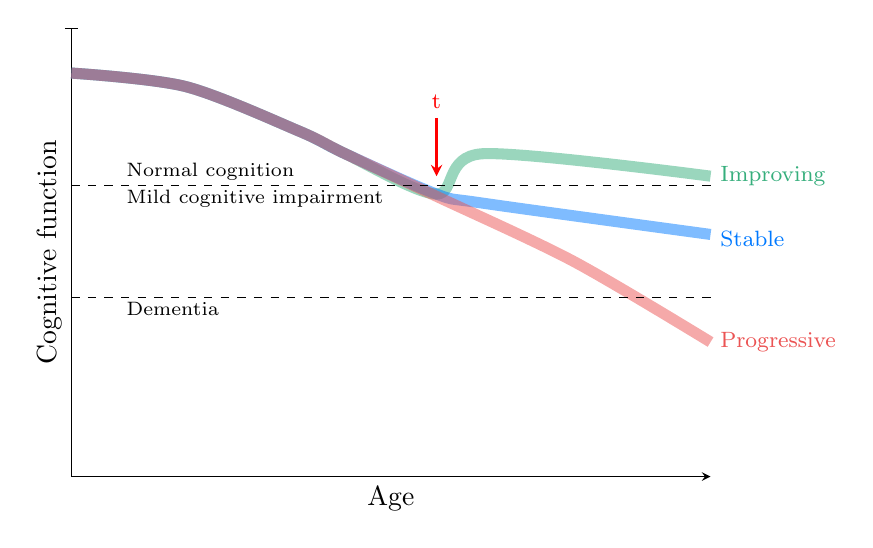
\begin{tikzpicture}
			\begin{axis}[
				height=0.6\textwidth,
				width=0.8\textwidth,
				xlabel={Age},
				ylabel={Cognitive function},
				ticks=none,
				axis x line=bottom,
				axis y line=left,
				y axis line style={-|},
				xmin=0,
				xmax=1.4,
				ymin=0,
				ymax=1,
				clip=false
			]
			\addplot[draw=healthy-default, smooth, line width=4pt, opacity=0.5] coordinates {
				(0, 0.9)
				(0.25, 0.87)
				(0.5, 0.77)
				(0.6, 0.72)
				(0.8, 0.63)
				(0.9, 0.72)
				(1.4, 0.67)
			};
			\addplot[draw=controls-default, smooth, line width=4pt, opacity=0.5] coordinates {
				(0, 0.9)
				(0.25, 0.87)
				(0.5, 0.77)
				(0.6, 0.72)
				(0.8, 0.63)
				(0.9, 0.61)
				(1.4, 0.54)
			};
			\addplot[draw=cases-default, smooth, line width=4pt, opacity=0.5] coordinates {
				(0, 0.9)
				(0.25, 0.87)
				(0.5, 0.77)
				(0.6, 0.72)
				(0.8, 0.625)
				(1.1, 0.48)
				(1.4, 0.3)
			};
			\addplot[dashed] coordinates {
				(0, 0.65)
				(1.4, 0.65)
			};
			\addplot[dashed] coordinates {
				(0, 0.4)
				(1.4, 0.4)
			};
			\node[anchor=south west] at (axis cs: 0.1, 0.64) {\scriptsize{Normal cognition}};
			\node[anchor=north west] at (axis cs: 0.1, 0.66) {\scriptsize{Mild cognitive impairment}};
			\node[anchor=north west] at (axis cs: 0.1, 0.41) {\scriptsize{Dementia}};
			\node[anchor=west] at (axis cs: 1.4, 0.67) {\textcolor{healthy-default}{\footnotesize{Improving}}};
			\node[anchor=west] at (axis cs: 1.4, 0.53) {\textcolor{controls-default}{\footnotesize{Stable}}};
			\node[anchor=west] at (axis cs: 1.4, 0.3) {\textcolor{cases-default}{\footnotesize{Progressive}}};
			\draw[-stealth, red, thick] (axis cs: 0.8, 0.8) -- (axis cs: 0.8, 0.67);
			\node[anchor=south] at (axis cs: 0.8, 0.8) {\textcolor{red}{\footnotesize{t}}};
			\end{axis}
		\end{tikzpicture}
		\vfill
	\end{frame}

	\begin{frame}{Paper 3: Explainable AI and dementia} % Prognosis
		\centering
		\vfill
		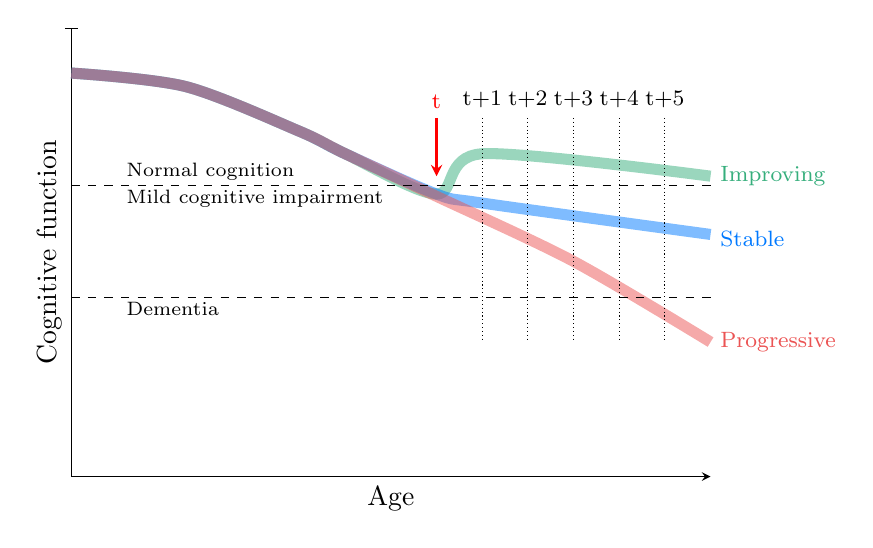
\begin{tikzpicture}
			\begin{axis}[
				height=0.6\textwidth,
				width=0.8\textwidth,
				xlabel={Age},
				ylabel={Cognitive function},
				ticks=none,
				axis x line=bottom,
				axis y line=left,
				y axis line style={-|},
				xmin=0,
				xmax=1.4,
				ymin=0,
				ymax=1,
				clip=false
			]
			\addplot[draw=healthy-default, smooth, line width=4pt, opacity=0.5] coordinates {
				(0, 0.9)
				(0.25, 0.87)
				(0.5, 0.77)
				(0.6, 0.72)
				(0.8, 0.63)
				(0.9, 0.72)
				(1.4, 0.67)
			};
			\addplot[draw=controls-default, smooth, line width=4pt, opacity=0.5] coordinates {
				(0, 0.9)
				(0.25, 0.87)
				(0.5, 0.77)
				(0.6, 0.72)
				(0.8, 0.63)
				(0.9, 0.61)
				(1.4, 0.54)
			};
			\addplot[draw=cases-default, smooth, line width=4pt, opacity=0.5] coordinates {
				(0, 0.9)
				(0.25, 0.87)
				(0.5, 0.77)
				(0.6, 0.72)
				(0.8, 0.625)
				(1.1, 0.48)
				(1.4, 0.3)
			};
			\addplot[dashed] coordinates {
				(0, 0.65)
				(1.4, 0.65)
			};
			\addplot[dashed] coordinates {
				(0, 0.4)
				(1.4, 0.4)
			};
			\node[anchor=south west] at (axis cs: 0.1, 0.64) {\scriptsize{Normal cognition}};
			\node[anchor=north west] at (axis cs: 0.1, 0.66) {\scriptsize{Mild cognitive impairment}};
			\node[anchor=north west] at (axis cs: 0.1, 0.41) {\scriptsize{Dementia}};
			\node[anchor=west] at (axis cs: 1.4, 0.67) {\textcolor{healthy-default}{\footnotesize{Improving}}};
			\node[anchor=west] at (axis cs: 1.4, 0.53) {\textcolor{controls-default}{\footnotesize{Stable}}};
			\node[anchor=west] at (axis cs: 1.4, 0.3) {\textcolor{cases-default}{\footnotesize{Progressive}}};
			\draw[-stealth, red, thick] (axis cs: 0.8, 0.8) -- (axis cs: 0.8, 0.67);
			\node[anchor=south] at (axis cs: 0.8, 0.8) {\textcolor{red}{\footnotesize{t}}};
			\draw[densely dotted] (axis cs: 0.9, 0.8) -- (axis cs: 0.9, 0.3);
			\draw[densely dotted] (axis cs: 1, 0.8) -- (axis cs: 1, 0.3);
			\draw[densely dotted] (axis cs: 1.1, 0.8) -- (axis cs: 1.1, 0.3);
			\draw[densely dotted] (axis cs: 1.2, 0.8) -- (axis cs: 1.2, 0.3);
			\draw[densely dotted] (axis cs: 1.3, 0.8) -- (axis cs: 1.3, 0.3);
			\node[anchor=south] at (axis cs: 0.9, 0.8) {\footnotesize{t+1}};
			\node[anchor=south] at (axis cs: 1, 0.8) {\footnotesize{t+2}};
			\node[anchor=south] at (axis cs: 1.1, 0.8) {\footnotesize{t+3}};
			\node[anchor=south] at (axis cs: 1.2, 0.8) {\footnotesize{t+4}};
			\node[anchor=south] at (axis cs: 1.3, 0.8) {\footnotesize{t+5}};
			\end{axis}
		\end{tikzpicture}
		\vfill
	\end{frame}

	\begin{frame}{Paper 3: Explainable AI and dementia} % Prognosis
		\centering
		\vfill
		\newsavebox{\resultsboxtwo}
			\sbox{\resultsboxtwo}{%
			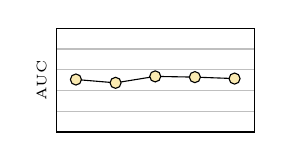
\begin{tikzpicture}
				\begin{axis}[
					height=2.9cm,
					width=4.1cm,
					xmajorticks=false,
					xmin=0.5,
					xmax=5.5,
					ymin=0,
					ymax=1,
					ylabel=\tiny{AUC},
					ymajorticks=false,
					ymajorgrids=true
				]
					\addplot[mark=*, draw=black, mark options={fill=baseline}] coordinates {
						(1, 0.506)
						(2, 0.474)
						(3, 0.536)
						(4, 0.529)
						(5, 0.515)
					};
				\end{axis}
			\end{tikzpicture}
		}
		\begin{tikzpicture}
			\begin{axis}[
				height=0.6\textwidth,
				width=0.8\textwidth,
				xlabel={Age},
				ylabel={Cognitive function},
				ticks=none,
				axis x line=bottom,
				axis y line=left,
				y axis line style={-|},
				xmin=0,
				xmax=1.4,
				ymin=0,
				ymax=1,
				clip=false
			]
			\addplot[draw=healthy-default, smooth, line width=4pt, opacity=0.5] coordinates {
				(0, 0.9)
				(0.25, 0.87)
				(0.5, 0.77)
				(0.6, 0.72)
				(0.8, 0.63)
				(0.9, 0.72)
				(1.4, 0.67)
			};
			\addplot[draw=controls-default, smooth, line width=4pt, opacity=0.5] coordinates {
				(0, 0.9)
				(0.25, 0.87)
				(0.5, 0.77)
				(0.6, 0.72)
				(0.8, 0.63)
				(0.9, 0.61)
				(1.4, 0.54)
			};
			\addplot[draw=cases-default, smooth, line width=4pt, opacity=0.5] coordinates {
				(0, 0.9)
				(0.25, 0.87)
				(0.5, 0.77)
				(0.6, 0.72)
				(0.8, 0.625)
				(1.1, 0.48)
				(1.4, 0.3)
			};
			\addplot[dashed] coordinates {
				(0, 0.65)
				(1.4, 0.65)
			};
			\addplot[dashed] coordinates {
				(0, 0.4)
				(1.4, 0.4)
			};
			\node[anchor=south west] at (axis cs: 0.1, 0.64) {\scriptsize{Normal cognition}};
			\node[anchor=north west] at (axis cs: 0.1, 0.66) {\scriptsize{Mild cognitive impairment}};
			\node[anchor=north west] at (axis cs: 0.1, 0.41) {\scriptsize{Dementia}};
			\node[anchor=west] at (axis cs: 1.4, 0.67) {\textcolor{healthy-default}{\footnotesize{Improving}}};
			\node[anchor=west] at (axis cs: 1.4, 0.53) {\textcolor{controls-default}{\footnotesize{Stable}}};
			\node[anchor=west] at (axis cs: 1.4, 0.3) {\textcolor{cases-default}{\footnotesize{Progressive}}};
			\draw[-stealth, red, thick] (axis cs: 0.8, 0.8) -- (axis cs: 0.8, 0.67);
			\node[anchor=south] at (axis cs: 0.8, 0.8) {\textcolor{red}{\footnotesize{t}}};
			\draw[densely dotted] (axis cs: 0.9, 0.8) -- (axis cs: 0.9, 0.3);
			\draw[densely dotted] (axis cs: 1, 0.8) -- (axis cs: 1, 0.3);
			\draw[densely dotted] (axis cs: 1.1, 0.8) -- (axis cs: 1.1, 0.3);
			\draw[densely dotted] (axis cs: 1.2, 0.8) -- (axis cs: 1.2, 0.3);
			\draw[densely dotted] (axis cs: 1.3, 0.8) -- (axis cs: 1.3, 0.3);
			\node[anchor=south] at (axis cs: 0.9, 0.8) {\footnotesize{t+1}};
			\node[anchor=south] at (axis cs: 1, 0.8) {\footnotesize{t+2}};
			\node[anchor=south] at (axis cs: 1.1, 0.8) {\footnotesize{t+3}};
			\node[anchor=south] at (axis cs: 1.2, 0.8) {\footnotesize{t+4}};
			\node[anchor=south] at (axis cs: 1.3, 0.8) {\footnotesize{t+5}};
			\node[] at (axis cs: 1.0755, 0.155) {
				\usebox{\resultsboxtwo}
			};
			\node[anchor=west] at (axis cs: 1.34, 0.158) {\footnotesize{0.51}};
			\end{axis}
		\end{tikzpicture}
		\vfill
	\end{frame}

	\begin{frame}{Paper 3: Explainable AI and dementia} % Prognosis
		\centering
		\vfill
		\newsavebox{\resultsboxone}
			\sbox{\resultsboxone}{%
			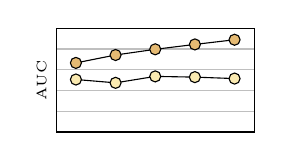
\begin{tikzpicture}
				\begin{axis}[
					height=2.9cm,
					width=4.1cm,
					xmajorticks=false,
					xmin=0.5,
					xmax=5.5,
					ymin=0,
					ymax=1,
					ylabel=\tiny{AUC},
					ymajorticks=false,
					ymajorgrids=true
				]
					\addplot[mark=*, draw=black, mark options={fill=baseline}] coordinates {
						(1, 0.506)
						(2, 0.474)
						(3, 0.536)
						(4, 0.529)
						(5, 0.515)
					};
					\addplot[mark=*, draw=black, mark options={fill=preds}] coordinates {
						(1, 0.666)
						(2, 0.742)
						(3, 0.797)
						(4, 0.844)
						(5, 0.889)
					};
				\end{axis}
			\end{tikzpicture}
		}
		\begin{tikzpicture}
			\begin{axis}[
				height=0.6\textwidth,
				width=0.8\textwidth,
				xlabel={Age},
				ylabel={Cognitive function},
				ticks=none,
				axis x line=bottom,
				axis y line=left,
				y axis line style={-|},
				xmin=0,
				xmax=1.4,
				ymin=0,
				ymax=1,
				clip=false
			]
			\addplot[draw=healthy-default, smooth, line width=4pt, opacity=0.5] coordinates {
				(0, 0.9)
				(0.25, 0.87)
				(0.5, 0.77)
				(0.6, 0.72)
				(0.8, 0.63)
				(0.9, 0.72)
				(1.4, 0.67)
			};
			\addplot[draw=controls-default, smooth, line width=4pt, opacity=0.5] coordinates {
				(0, 0.9)
				(0.25, 0.87)
				(0.5, 0.77)
				(0.6, 0.72)
				(0.8, 0.63)
				(0.9, 0.61)
				(1.4, 0.54)
			};
			\addplot[draw=cases-default, smooth, line width=4pt, opacity=0.5] coordinates {
				(0, 0.9)
				(0.25, 0.87)
				(0.5, 0.77)
				(0.6, 0.72)
				(0.8, 0.625)
				(1.1, 0.48)
				(1.4, 0.3)
			};
			\addplot[dashed] coordinates {
				(0, 0.65)
				(1.4, 0.65)
			};
			\addplot[dashed] coordinates {
				(0, 0.4)
				(1.4, 0.4)
			};
			\node[anchor=south west] at (axis cs: 0.1, 0.64) {\scriptsize{Normal cognition}};
			\node[anchor=north west] at (axis cs: 0.1, 0.66) {\scriptsize{Mild cognitive impairment}};
			\node[anchor=north west] at (axis cs: 0.1, 0.41) {\scriptsize{Dementia}};
			\node[anchor=west] at (axis cs: 1.4, 0.67) {\textcolor{healthy-default}{\footnotesize{Improving}}};
			\node[anchor=west] at (axis cs: 1.4, 0.53) {\textcolor{controls-default}{\footnotesize{Stable}}};
			\node[anchor=west] at (axis cs: 1.4, 0.3) {\textcolor{cases-default}{\footnotesize{Progressive}}};
			\draw[-stealth, red, thick] (axis cs: 0.8, 0.8) -- (axis cs: 0.8, 0.67);
			\node[anchor=south] at (axis cs: 0.8, 0.8) {\textcolor{red}{\footnotesize{t}}};
			\draw[densely dotted] (axis cs: 0.9, 0.8) -- (axis cs: 0.9, 0.3);
			\draw[densely dotted] (axis cs: 1, 0.8) -- (axis cs: 1, 0.3);
			\draw[densely dotted] (axis cs: 1.1, 0.8) -- (axis cs: 1.1, 0.3);
			\draw[densely dotted] (axis cs: 1.2, 0.8) -- (axis cs: 1.2, 0.3);
			\draw[densely dotted] (axis cs: 1.3, 0.8) -- (axis cs: 1.3, 0.3);
			\node[anchor=south] at (axis cs: 0.9, 0.8) {\footnotesize{t+1}};
			\node[anchor=south] at (axis cs: 1, 0.8) {\footnotesize{t+2}};
			\node[anchor=south] at (axis cs: 1.1, 0.8) {\footnotesize{t+3}};
			\node[anchor=south] at (axis cs: 1.2, 0.8) {\footnotesize{t+4}};
			\node[anchor=south] at (axis cs: 1.3, 0.8) {\footnotesize{t+5}};
			\node[] at (axis cs: 1.0755, 0.155) {
				\usebox{\resultsboxone}
			};
			\node[anchor=west] at (axis cs: 1.34, 0.261) {\footnotesize{0.88}};
			\end{axis}
		\end{tikzpicture}
		\vfill
	\end{frame}

	\begin{frame}{Paper 3: Explainable AI and dementia} % Prognosis
		\centering
		\vfill
		\newsavebox{\resultsbox}
			\sbox{\resultsbox}{%
			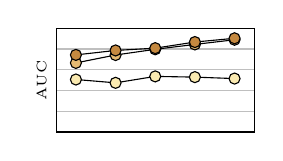
\begin{tikzpicture}
				\begin{axis}[
					height=2.9cm,
					width=4.1cm,
					xmajorticks=false,
					xmin=0.5,
					xmax=5.5,
					ymin=0,
					ymax=1,
					ylabel=\tiny{AUC},
					ymajorticks=false,
					ymajorgrids=true
				]
					\addplot[mark=*, draw=black, mark options={fill=baseline}] coordinates {
						(1, 0.506)
						(2, 0.474)
						(3, 0.536)
						(4, 0.529)
						(5, 0.515)
					};
					\addplot[mark=*, draw=black, mark options={fill=preds}] coordinates {
						(1, 0.666)
						(2, 0.742)
						(3, 0.797)
						(4, 0.844)
						(5, 0.889)
					};
					\addplot[mark=*, draw=black, mark options={fill=maps}] coordinates {
						(1, 0.743)
						(2, 0.786)
						(3, 0.808)
						(4, 0.867)
						(5, 0.903)
					};
				\end{axis}
			\end{tikzpicture}
		}
		\begin{tikzpicture}
			\begin{axis}[
				height=0.6\textwidth,
				width=0.8\textwidth,
				xlabel={Age},
				ylabel={Cognitive function},
				ticks=none,
				axis x line=bottom,
				axis y line=left,
				y axis line style={-|},
				xmin=0,
				xmax=1.4,
				ymin=0,
				ymax=1,
				clip=false
			]
			\addplot[draw=healthy-default, smooth, line width=4pt, opacity=0.5] coordinates {
				(0, 0.9)
				(0.25, 0.87)
				(0.5, 0.77)
				(0.6, 0.72)
				(0.8, 0.63)
				(0.9, 0.72)
				(1.4, 0.67)
			};
			\addplot[draw=controls-default, smooth, line width=4pt, opacity=0.5] coordinates {
				(0, 0.9)
				(0.25, 0.87)
				(0.5, 0.77)
				(0.6, 0.72)
				(0.8, 0.63)
				(0.9, 0.61)
				(1.4, 0.54)
			};
			\addplot[draw=cases-default, smooth, line width=4pt, opacity=0.5] coordinates {
				(0, 0.9)
				(0.25, 0.87)
				(0.5, 0.77)
				(0.6, 0.72)
				(0.8, 0.625)
				(1.1, 0.48)
				(1.4, 0.3)
			};
			\addplot[dashed] coordinates {
				(0, 0.65)
				(1.4, 0.65)
			};
			\addplot[dashed] coordinates {
				(0, 0.4)
				(1.4, 0.4)
			};
			\node[anchor=south west] at (axis cs: 0.1, 0.64) {\scriptsize{Normal cognition}};
			\node[anchor=north west] at (axis cs: 0.1, 0.66) {\scriptsize{Mild cognitive impairment}};
			\node[anchor=north west] at (axis cs: 0.1, 0.41) {\scriptsize{Dementia}};
			\node[anchor=west] at (axis cs: 1.4, 0.67) {\textcolor{healthy-default}{\footnotesize{Improving}}};
			\node[anchor=west] at (axis cs: 1.4, 0.53) {\textcolor{controls-default}{\footnotesize{Stable}}};
			\node[anchor=west] at (axis cs: 1.4, 0.3) {\textcolor{cases-default}{\footnotesize{Progressive}}};
			\draw[-stealth, red, thick] (axis cs: 0.8, 0.8) -- (axis cs: 0.8, 0.67);
			\node[anchor=south] at (axis cs: 0.8, 0.8) {\textcolor{red}{\footnotesize{t}}};
			\draw[densely dotted] (axis cs: 0.9, 0.8) -- (axis cs: 0.9, 0.3);
			\draw[densely dotted] (axis cs: 1, 0.8) -- (axis cs: 1, 0.3);
			\draw[densely dotted] (axis cs: 1.1, 0.8) -- (axis cs: 1.1, 0.3);
			\draw[densely dotted] (axis cs: 1.2, 0.8) -- (axis cs: 1.2, 0.3);
			\draw[densely dotted] (axis cs: 1.3, 0.8) -- (axis cs: 1.3, 0.3);
			\node[anchor=south] at (axis cs: 0.9, 0.8) {\footnotesize{t+1}};
			\node[anchor=south] at (axis cs: 1, 0.8) {\footnotesize{t+2}};
			\node[anchor=south] at (axis cs: 1.1, 0.8) {\footnotesize{t+3}};
			\node[anchor=south] at (axis cs: 1.2, 0.8) {\footnotesize{t+4}};
			\node[anchor=south] at (axis cs: 1.3, 0.8) {\footnotesize{t+5}};
			\node[] at (axis cs: 1.0755, 0.155) {
				\usebox{\resultsbox}
			};
			\node[anchor=west] at (axis cs: 1.34, 0.262) {\footnotesize{0.90}};
			\end{axis}
		\end{tikzpicture}
		\vfill
	\end{frame}

	\begin{frame}{Paper 3: Explainable AI and dementia} % Correlations
		\newcommand{\mriwidth}{2.2cm}
        \newcommand{\gap}{0.00cm}

        \newcommand{\correlationplot}[4]{
            \begin{tikzpicture}
                \begin{axis}[
                    height=1.71 * \mriwidth,
                    width=1.71 * \mriwidth,
                    xmajorticks=false,
                    ylabel=####3,
                    ytick={0, 2, 4, 6, 8},
                    yticklabels=####2,
                    xmin=-1,
                    xmax=17,
                    ymin=0,
                    ymax=9,
                    every tick label/.append style={font=\tiny},
                    ytick pos=left,
                    scatter/classes={
                        ADNI_EF={color0, draw=black},
                        ADNI_MEM={color1, draw=black},
                        CDCARE={color2, draw=black},
                        CDCOMMUN={color3, draw=black},
                        CDGLOBAL={color4, draw=black},
                        CDHOME={color5, draw=black},
                        CDJUDGE={color6, draw=black},
                        CDMEMORY={color7, draw=black},
                        CDORIENT={color8, draw=black},
                        FAQTOTAL={color9, draw=black},
                        GDTOTAL={color10, draw=black},
                        MMSCORE={color11, draw=black},
                        NPISCORE={color12, draw=black},
                        PHC_EXF={color13, draw=black},
                        PHC_LAN={color14, draw=black},
                        PHC_MEM={color15, draw=black},
                        PHC_VSP={color16, draw=black}
                    },
                    y label style={at={(-0.1,0.5)}},
                    ymajorgrids=true,
                    ytick style={draw=none},
                    clip=false,
                    grid style={draw=gray!20},
                    axis line style={draw=gray!70}
                ]
                    \addplot[
                        only marks,
                        scatter,
                        scatter src=explicit symbolic
                    ] table [
                        col sep=comma,
                        x=index,
                        y=component_####1,
                        meta=symptom
                    ] {data/correlations.csv};
                    \addplot[dashed,red, thick] coordinates {
                        (-1, 2.76)
                        (17, 2.76)
                    };
                    ####4
                \end{axis}
            \end{tikzpicture}
        }

        \newsavebox{\firstcorrelations}
        \sbox{\firstcorrelations}{%
            \correlationplot{0}{{0, 2, 4, 6, 8}}{\scriptsize{$-log_{10}(p)$}}{
                \node[] at (axis cs: 14, 6.09) {\tiny{PHC\_LAN}};
            }
        }
        \newsavebox{\secondcorrelations}
        \sbox{\secondcorrelations}{%
            \correlationplot{1}{{,,}}{{}}{
                \node[] at (axis cs: 9, 3.64) {\tiny{FAQTOTAL}};
            }
        }
        \newsavebox{\thirdcorrelations}
        \sbox{\thirdcorrelations}{%
            \correlationplot{2}{{,,}}{{}}{
                \node[] at (axis cs: 0, 6.34) {\tiny{ADNI\_EF}};
                \node[] at (axis cs: 13, 7.85) {\tiny{PHC\_EXF}};
            }
        }
        \newsavebox{\fourthcorrelations}
        \sbox{\fourthcorrelations}{%
            \correlationplot{3}{{,,}}{{}}{
                \node[] at (axis cs: 0, 8.92) {\tiny{ADNI\_EF}};
                \node[] at (axis cs: 13, 8.65) {\tiny{PHC\_EXF}};
                \node[] at (axis cs: 14, 5.84) {\tiny{PHC\_LAN}};
                \node[] at (axis cs: 6, 5.08) {\tiny{CDJUDGE}};
                \node[] at (axis cs: 11, 3.89) {\tiny{MMSCORE}};
            }
        }

        \begin{tikzpicture}
            \node[] (first) at (0, 0) {
                \includegraphics[
                    width=\mriwidth,
                    clip=true,
                    trim = 192mm 232mm 0mm 0mm
                ]{data/components/component_0.png}
            };
            \node[anchor=north west] (first-correlation) at ($ (first.south west) + (-0.73, 0.1) $) {
                \usebox{\firstcorrelations}
            };

            \node[anchor=west] (second) at ($ (first.east) + (\gap, 0) $) {
                \includegraphics[
                    width=\mriwidth,
                    clip=true,
                    trim = 192mm 232mm 0mm 0mm
                ]{data/components/component_1.png}
            };
            \node[anchor=north west] (second-correlation) at ($ (first-correlation.north east) - (0.56, 0) $) {
                \usebox{\secondcorrelations}
            };

            \node[anchor=west] (third) at ($ (second.east) + (\gap, 0) $) {
                \includegraphics[
                    width=\mriwidth,
                    clip=true,
                    trim = 192mm 232mm 0mm 0mm
                ]{data/components/component_2.png}
            };
            \node[anchor=north west] (third-correlation) at ($ (second-correlation.north east) - (0.56, 0) $) {
                \usebox{\thirdcorrelations}
            };

            \node[anchor=west] (fourth) at ($ (third.east) + (\gap, 0) $) {
                \includegraphics[
                    width=\mriwidth,
                    clip=true,
                    trim = 192mm 232mm 0mm 0mm
                ]{data/components/component_3.png}
            };
            \node[anchor=north west] (fourth-correlation) at ($ (third-correlation.north east) - (0.56, -0.16) $) {
                \usebox{\fourthcorrelations}
            };
        \end{tikzpicture}
	\end{frame}

	\begin{frame}{Practical stuff}
		\begin{itemize}
			\item[\textcolor{green}{\checkmark}] 35/30 credits
			\item[\textcolor{green}{\checkmark}] Presented at conference
			\item[\textcolor{orange}{?}] ?/? teaching hours (PSY9511 this fall)
			\item[\textcolor{green}{\checkmark}] Public dissemination
			\item[\textcolor{green}{\checkmark}] Open source contributions
		\end{itemize}
	\end{frame}
\end{document}
